%!TEX root = main.tex

%Recall that the definition of $\STK$-dominating $\LMAMASS$, then we let $\tau= A\xrightarrow{\startactivity(\bot)}B$ and let $\rho = (S_1, \cdots, S_n)$ be the current configuration for some $n \ge 1$ and $\topact(\rho) = A$. 

%we define the semantics of $\STK$-dominating $\LMAMASS$ as follows:
%\begin{itemize}
%    \item If $\lmd(B) = \STD$, then $\rho' = \push(\rho, B)$,
%    \item If $\lmd(B) = \STK$, then 
%    \begin{itemize}
%        \item if $\gettsk(\rho, B) = S_i$ for some $i\in[n]$, then
%        \begin{itemize}
 %           \item if $B \not \in S_i$, then $\rho' = \push(\mvtsktop(\rho, i), B)$,
 %           \item if $B  \in S_i$, 	then $\rho' =  \clrtop(\mvtsktop(\rho, i), B)$,
 %       \end{itemize}
%    \item if $\gettsk(\rho, B) = *$, then $\rho' = \newtsk(\rho, B)$.
%    \end{itemize}
%\end{itemize}

In this section, we first define the semantics of $\LMAMASS$, then show how to solve the configuration reachability problem of $\STK$-dominating $\LMAMASS$. 

%%%%%%%%%%%%%%%%%%%%%%%%%%%%%%%%%%%%%%%%%%%%%%%

%!TEX root = main.tex

\subsection{Semantics of $\LMAMASS$} \label{sect:semlmamass}

%We start with the semantics of $\LMAMASS$ and assume that $\Mm$ is an $\LMAMASS$. 

%Before presenting the formal semantics of $\LMAMASS$, let us describe the intuitions behind it.

%
\noindent\emph{Intuitions.}  We first explain the intuitions of the four launch modes. 

\begin{itemize}
	\item  $\STD$: When a new $\STD$-activity is started, it is pushed to the top task. 
	%
	\item $\STP$: When a new $\STP$-activity is started, if the activity is already at the top of the top task, it will reuse this activity. Otherwise, a new activity will be pushed into the top task.
	%
	\item $\STK$: When a new $\STK$-activity is started, it will create the activity at the root of a new task or locate the activity on an existing task with the same affinity. If the activity already exists, then all the activities above it are removed from the task. Otherwise, a new activity will be pushed into the task.
	%
	\item $\SIT$: 
	Similar to $\STK$, but if such an activity already exists, it will reuse this activity, moreover, there is only one activity in the task which was created by starting the same activity.
\end{itemize}




%Via extensive experiments, we identify a crucial notion, i.e., task affinity of tasks, which plays a pivotal role in such a mechanism.
When an activity is launched, it may not be put in the top task, in which case  
%When an activity $B$ is launched and not going to be put in the top task, 
the following rules are used to determine which task will it be allocated. 
\begin{itemize}
	\item In case $\lmd(B) \neq \SIT$, if there is a non-$\SIT$-task whose task affinity is the same as $B$, then $B$ will be put on the task; otherwise, a new task will be created to hold $B$.
	
	\item In case $\lmd(B) = \SIT$,    if there is any task whose bottom activity is $B$ (actually $B$ is the only activity in the task), then the task will be moved to the top; otherwise, a new task is created to hold $B$.
\end{itemize}

%%%%%%%%%%%%%%%%%%%%%%%%%%%%%%%%%%%%%%%%%%%%%%%
\noindent\textbf{Caveat.} The intuition is stated to facilitate readers to under the transitions rules at a high level. They are not necessarily precise at a formal level. For instance, when a new $\STD$-activity is stated by an $\SIT$-activity, the $\STD$-activity will not necessarily be pushed to the top task. 
%Task allocation mechanism is to specify to which task will it be allocated when an activity is launched. 
%%%%%%%%%%%%%%%%%%%%%%%%%%%%%%%%%%%%%%%%%%%%%%
%!TEX root = main.tex

We introduce some auxiliary functions and predicates to be used in the formal semantics of $\LMAMASS$.

%\begin{figure}
%	\begin{center}
	%\begin{tabular}{l}
	%\hline\\
	% $\topact(S) = A_1$, $\btmact(S) = A_m$\\
	%$\toptsk(\rho) = S_1$, $\topact(\rho) = \topact(\toptsk(\rho))$\\
	%$\push(\rho, B) = (([B]\cdot S_1,\aname_1),(S_2,\aname_2),\cdots,(S_n,\aname_n))$\\
	%\end{tabular}	
	%\caption{Auxiliary functions and predicates} \label{fig:syntax}
	%\end{center}
	%\end{figure}
	
	\paragraph{Auxiliary functions and predicates} 
	%To specify the transition relation precisely and concisely, we define the following functions and predicates. 
	Let $\rho= ((S_1,\aname_1),\cdots, (S_n,\aname_n))$ be a configuration and $S=[A_1, \cdots, A_m]$ be a task. 
	\begin{itemize}
		\item $\topact(S) = A_1$, $\btmact(S) = A_m$,
		\item $\toptsk(\rho) = S_1$, $\topact(\rho) = \topact(\toptsk(\rho))$, 
		\item $\push(\rho, B) = (([B]\cdot S_1,\aname_1),(S_2,\aname_2),\cdots,(S_n,\aname_n))$,
		\item $\Pop(\rho) = ((S_1',\aname_1),(S_2,\aname_2), \cdots, (S_n,\aname_n))$ if $S_1=[B]\cdot S_1'$ for some $B\in\act$ and $S_1'\in\act^+$,\\ $\Pop(\rho) = ((S_2,\aname_2),\cdots,(S_n,\aname_n))$ otherwise,
		% \item $\mvacttop(\rho, B) = ([B]\cdot S_1'\cdot S_1'', S_2, \cdots, S_n)$, if $S_1=S_1'\cdot[B]\cdot S_1''$ with $S_1'\in (\act\setminus\{B\})^*$,
		\item $\clrtop(\rho, B) = (([B]\cdot S_1'',\aname_1), (S_2,\aname_2), \cdots, (S_n,\aname_n))$, if $S_1=S_1'\cdot[B]\cdot S_1''$ with $S_1'\in (\act\setminus\{B\})^*$,
		% \item $\clrtsk(\rho, B) = ([B], S_2, \cdots, S_n)$,
		\item $\newtsk(\rho, B) = (([B],\aft(B)), S_1, \cdots, S_n)$,
		\item $\mvtsktop(\rho, i)$ is defined as 
		$$((S_i,\aname_i), (S_1,\aname_1), \cdots, (S_{i-1},\aname_{i-1}), (S_{i+1},\aname_{i+1}), \cdots, (S_n,\aname_n)),$$
		% \item $\gettsk(\rho, B) = S_i$ such that $i \in [n]$ is the \emph{minimum} index satisfying $\aft(A_i)=\aft(B)$, if such an index $i$ exists; $\gettsk(\rho, B) = *$ otherwise.
		%
		\item $\gettsk(\rho, B)$ is defined as follows,
		\begin{itemize}
			\item if $\lmd(B)\neq\singleinstance$, $\aname_i=\aft(B)$ and $\lmd(\btmact(S_i)) \neq \singleinstance$ for some $i \in [n]$,  then $\gettsk(\rho, B) = S_i$, otherwise, $\gettsk(\rho, B) = *$.
			\item if $\lmd(B) = \singleinstance$, $\btmact(S_i)=B$ for some $i \in [n]$, then $\gettsk(\rho, B) = S_i$, otherwise, $\gettsk(\rho, B) = *$.
		\end{itemize}
	\end{itemize}
	
Note that $\gettsk(\rho, B)$ formalizes the aforementioned task allocation mechanism and the fact that the task affinities of two different non-$\SIT$ tasks are distinct guarantees that the function $\gettsk(\rho, B)$ is well-defined. 
	
	%We are ready to define the semantics of $\LMAMASS$ as the transition relation $\xrightarrow[\Mm]{}$ in the sequel. 
	


\smallskip

\paragraph{Transition rules} 


Let $\rho = ((S_1,\aname_1),\cdots,(S_n,\aname_n))$ be the current configuration for some $n \ge 1$ and $\topact(\rho) = A$. Moreover, let $S_1 = [A_1',\cdots,A_m']$. Evidently, $A = A_1'$. We show how $\rho'$ can be obtained from $\rho$ and $\tau$.
	
	If $\tau = \back$, then $\rho' = \Pop(\rho)$. 
	
	Then consider $\tau = A\xrightarrow{\startactivity(\bot)}B$.
	
	% The definition of $\rho \xrightarrow[\Mm]{\tau} \rho'$ for $\tau= A\xrightarrow{\startactivity(\phi)}B$ is much more complicated. 
	% Let $\tau= A\xrightarrow{\startactivity(\phi)}B$ and $\rho = (S_1, \cdots, S_n)$ be the current configuration for some $n \ge 1$ such that $\topact(\rho) = A$. 
	% To ease the reading, we first consider the simpler cases that $\tau$ is from $\LMAMASS$ or $\IFAMASS$,  then consider the more general case that $\tau$ is from $\AMASS$. 
	
	
	% As the semantics of $\Mm$ are highly complex, we will formalize the semantics step by step. Firstly, we consider the case without the intent flag, then we consider the case with only the intent flag, and finally we consider the complete semantics.
	
	
	
	%\fcolorbox{red}{yellow}{%
		%	\minipage[t]{\dimexpr0.48\linewidth-2\fboxsep-2\fboxrule\relax}
		%	If $\lmd(A) \neq \SIT$, then $\rho'= \push(\rho,B)$.
		%	\endminipage}\hfill
	%\fcolorbox{red}{yellow}{%
		%	\minipage[t]{\dimexpr0.48\linewidth-2\fboxsep-2\fboxrule\relax}
		%	If $\lmd(A) = \SIT$, then
		%	\begin{itemize}
			%		\item if $\gettsk(\rho, B)=S_i$ for some $i\in[n]$,  then 
			%		$$\rho'=\push(\mvtsktop(\rho, i),B),$$
			%		\item if $\gettsk(\rho, B)=*$, then $\rho'= \newtsk(\rho,B )$.
			%	\end{itemize}
		%	\endminipage}

\medskip	
	
	\noindent \fbox{\fbox{$\lmd(B) = \STD$}}
	
	%\tcbset{width=(\linewidth-2mm)/2,before=,after=\hfill,arc=0mm,
		%	colframe=blue!75!black,colback=white,fonttitle=\bfseries}
	%title=Box \thetcbrasternum,
	%enhanced,size=small] %colframe=red!50!black,colback=red!10!white]
%	\begin{tcolorbox}[width=0.4\linewidth, title={$\lmd(A) = \SIT$}]
%		$\rho'= \push(\rho,B)$
%	\end{tcolorbox} \hfill
%	\begin{tcolorbox}[width=0.6\linewidth, title={$\lmd(A) \neq \SIT$}]
%		\begin{itemize}
%			\item if $\gettsk(\rho, B)=S_i$ for some $i\in[n]$,  then 
%			$\rho'=\push(\mvtsktop(\rho, i),B),$
%			\item	if $\gettsk(\rho, B)=*$, then $\rho'= \newtsk(\rho,B )$.
%		\end{itemize}
%	\end{tcolorbox}	
	
\begin{itemize}
				\item If $\lmd(A) \neq \SIT$, then $\rho'= \push(\rho,B)$.
				%
				\item If $\lmd(A) = \SIT$, then
		    		\begin{itemize}
			    			\item if $\gettsk(\rho, B)=S_i$ for some $i\in[n]$,  then 
						$$\rho'=\push(\mvtsktop(\rho, i),B),$$
			    			\item if $\gettsk(\rho, B)=*$, then $\rho'= \newtsk(\rho,B )$.
			    		\end{itemize}
\end{itemize}
	
	
	
	\noindent \fbox{\fbox{$\lmd(B) = \STP$}}
	\begin{itemize}
		\item  If $\lmd(A) \neq \SIT$ and $A \neq B$, then $\rho' = \push(\rho,B)$.
		%
		\item  If $\lmd(A) \neq \SIT$ and $A = B$, then $\rho' =  \rho$.
		%
		\item If $\lmd(A) = \SIT$, then
		\begin{itemize}
			\item if $\gettsk(\rho, B)=S_i$ for some $i\in[n]$,  then
			\begin{itemize}
				\item if $\topact(S_i)\neq B$, then 
				$$\rho'=\push(\mvtsktop(\rho, i),B),$$
				\item if $\topact(S_i)= B$, then $\rho'=\mvtsktop(\rho, i),$
			\end{itemize}
			\item if $\gettsk(\rho, B)=*$, then $\rho'= \newtsk(\rho,B )$.
		\end{itemize}
	\end{itemize}
	
	\noindent \fbox{\fbox{$\lmd(B) = \singletask$}}
	\begin{itemize}
		\item If $\gettsk(\rho, B) = S_i$ for some $i\in[n]$, then
		\begin{itemize}
			\item if $B \not \in S_i$, then $\rho' = \push(\mvtsktop(\rho, i), B)$,
			\item if $B  \in S_i$, 	then $\rho' =  \clrtop(\mvtsktop(\rho, i), B)$.
		\end{itemize}
		\item If $\gettsk(\rho, B) = *$, then $\rho' = \newtsk(\rho, B)$.
	\end{itemize}
	
	\noindent \fbox{\fbox{$\lmd(B) = \SIT$}}
	\begin{itemize}
		\item If $\gettsk(\rho, B) = S_i$ for some $i \in [n]$, then $\rho' = \mvtsktop(\rho, i)$.
		\item If $\gettsk(\rho, B) = *$, then $\rho' = \newtsk(\rho, B)$.
	\end{itemize}
	
	This concludes the definition of the transition rules for $\LMAMASS$. 
	
	
	
%	%%%%%%%%%%%%%%%%
%	\tl{to see where to put this.} Moreover, it is not hard to verify that the transition relation $\xrightarrow[\Mm]{\tau}$ preserves the invariant of configurations, that is, if $\rho$ satisfies that the task affinities of every two non-$\singleinstance$ tasks are different, and $\rho \xrightarrow[\Mm]{\tau} \rho'$ for some $\tau$, then $\rho'$ satisfies this invariant as well. 
%	%%%%%%%%%%%%%%%%%%%%%%

It is not hard to verify that the transition relation $\xrightarrow[\Mm]{}$ %preserves the invariant of configurations, that is, 
	satisfies that, if the task affinities of two non-$\singleinstance$ tasks are different in $\rho$ and $\rho \xrightarrow[\Mm]{\tau} \rho'$ for some $\tau$, then the task affinities of two non-$\singleinstance$ tasks are different in $\rho'$. This justifies the second constraint in the definition of configurations in the previous section. 
	
	
	%%%%%%%%%%%%%%%%%%%%%%%%%%%%%%%%%%%%%%%%%% example %%%%%%%%%%%%%%%%%%%%%%%%%%%%%%%%%%%%%%%%%%%%%%%%
	We use the following example to illustrate the semantics.
	\begin{example}
		Let $\Mm = (\act,A,\lmd,\aft,\Delta)$ be an $\LMAMASS$, where $\act = \{A,B,C,D\}$, the functions $\lmd$ and $\aft$ are defined in Table~\ref{tab-attribute}.
		\begin{table}[htbp]
			\begin{center}
				\begin{tabular}{|c|c|c|c|c|c|}
					\hline
					Activity & $\lmd$ & $\aft$\\
					\hline
					$A$ & $\STD$ & 1 \\
					\hline
					$B$ & $\STK$ & 2 \\
					\hline
					$C$ & $\STP$ & 2 \\
					\hline
					$D$ & $\SIT$ & 2 \\
					\hline
				\end{tabular}
				\caption{Attributes of activities}
				\label{tab-attribute}
			\end{center}
		\end{table}
		
		Moreover, $\Delta = \{\tau_1, \tau_2, \tau_3, \tau_4, \tau_5\}$, where 
		$\tau_1 = A \xrightarrow{\startactivity(\bot)} B$,
		$\tau_2 = B \xrightarrow{\startactivity(\bot)} C$,
		$\tau_3 = C \xrightarrow{\startactivity(\bot)} D$,
		$\tau_4 = D \xrightarrow{\startactivity(\bot)} B$,
		$\tau_5 = D \xrightarrow{\startactivity(\bot)} C$.
		% $\rho_0 = (([D_1],D_1,1))$, and\\
		Then the configurations that are reachable from the initial configuration $(([A], 1))$ by executing the transition rules from $\Delta$ are illustrated in Figure~\ref{lmasm-example}, where the vertices denote the configurations and the edges denote the elements of $\xrightarrow[\Mm]{}$. 
		For instance, 
		\begin{itemize}
			\item if $A \xrightarrow{\startactivity(\bot)} B$ is applied to the configuration $(([A], 1))$, then a new task $([B],2)$ is created, since $\lmd(B) = \STK$ and $\gettsk((([A],1)), B) = *$, resulting in the configuration $(([B],2),([A],1))$,
			%
			% \item if $B \xrightarrow{\startactivity(\bot)} B$ is applied to the configuration $(([BA], 1))$, then $B$ will not be pushed, since $\lmd(B) = \STP$ and the top activity of the top task is $B$, 
			%
			\item if $B \xrightarrow{\startactivity(\bot)} C$ is applied to the configuration $(([B],2),([A],1))$, then $C$ is pushed, since $\lmd(C) = \STP$ and $B\neq C$, resulting in the configuration $(([CB],2),([A],1))$,
			%
			\item if $C \xrightarrow{\startactivity(\bot)} D$ is applied to the configuration $(([CB],2),([A],1))$, then a new task $([D], 2)$ is created, since 
			$$\lmd(D) = \SIT \mbox{ and } \gettsk((([CB],2),([A],1)), D) = *,$$ 
			resulting in the configuration $(([D],2),([CB],2),([A],1))$,
			%
			\item if $D \xrightarrow{\startactivity(\bot)} B$ is applied to the configuration $(([D],2),([CB],2),([A],1))$, then the task $([CB],2)$ is moved to the top and all the activities above $B$, which is $C$ here, are removed from the task, since $\lmd(B) = \STK$, 
			$$\gettsk((([D],2),([CB],2),([A],1)), B) = ([CB],2)$$
			and $B$ occurs in $([CB], 2)$, resulting in the configuration 
			$$(([B],2),([D],2),([A],1)),$$
			%
			\item if $D \xrightarrow{\startactivity(\bot)} C$ is applied to the configuration $(([D],2),([CB],2),([A],1))$, then the task $([CB],2)$ is moved to the top, but $C$ will not be pushed, since $\lmd(C) = \STP$, $\lmd(D) = \SIT$,
			$$\gettsk((([D],2),([CB],2),([A],1)), C) = ([CB],2)$$
			and $C$ is the top activity of $([CB], 2)$, resulting in the configuration $(([CB],2),([D],2),([A],1))$,
			%
			\item if $C \xrightarrow{\startactivity(\bot)} D$ is applied to the configuration $(([CB],2),([D],2),([A],1))$, then the task $([D],2)$ is moved to the top, since $\lmd(D) = \SIT$ and
			$$\gettsk((([CB],2),([D],2),([A],1)), D) = ([D],2)$$
			resulting in the configuration $(([D],2),([CB],2),([A],1))$.
		\end{itemize}
		Note that for $\Mm$, there are only finitely many configurations reachable from the initial configuration, which may not be the case for $\LMAMASS$ in general.  
		% $(([D_1],D_1,1))$\\
		% $\xrightarrow[\tau_1]{\Mm}(([P_1D_1],D_1,1))$\\
		% $\xrightarrow[\tau_2]{\Mm}(([P_1D_1],D_1,1))$\\
		% $\xrightarrow[\tau_3]{\Mm}(([K_2],K_2,0),([P_1D_1],D_1,1))$\\
		% $\xrightarrow[\tau_4]{\Mm}(([D_1K_2],K_2,0),([P_1D_1],D_1,1))$\\
		% $\xrightarrow[\tau_5]{\Mm}(([T_2],T_2,0),([D_1K_2],K_2,0),([P_1D_1],D_1,1))$\\
		% $\xrightarrow[\tau_6]{\Mm}(([K_2],K_2,0),([T_2],T_2,0),([P_1D_1],D_1,1))$\\
		
		\begin{figure}
			% \vspace{-3mm}
			\centering
			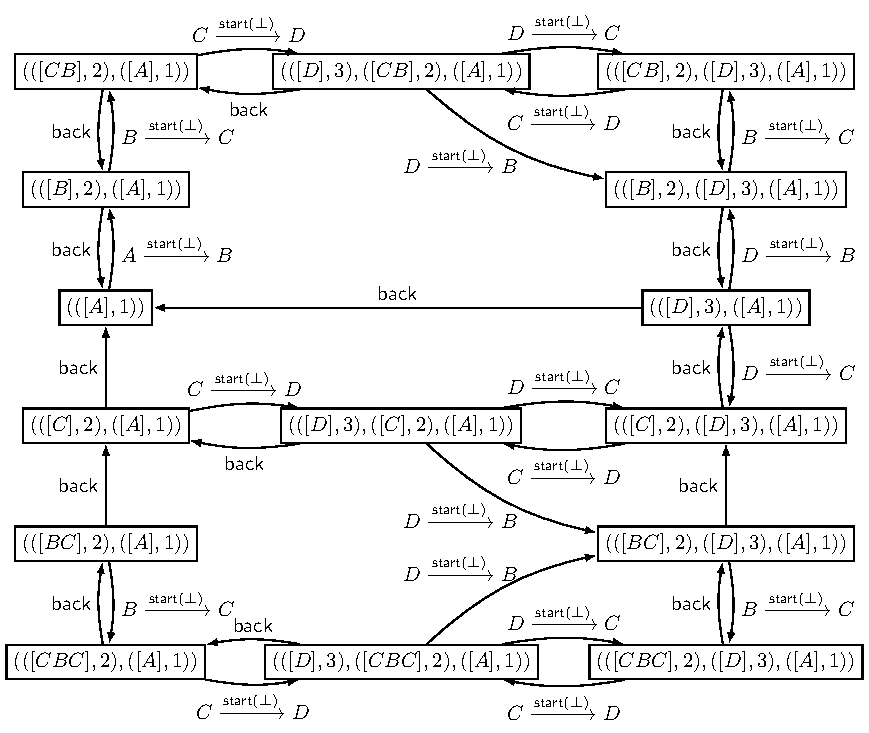
\includegraphics[scale = 0.75]{lmasm-example.pdf}
			\caption{Configurations reachable from the initial configuration $(([A], 1))$ in $\LMAMASS$}
			%in $\phi$
			% \vspace{-6mm}	
			\label{lmasm-example}
		\end{figure}
Finally, if we remove $\tau_5$ from $\Mm$, let $\Mm'$ denote the resulting $\LMAMASS$, then $\Mm'$ is an $\STK$-dominating $\LMAMASS$: In $\Mm'$, there is only one $\STK$-activity, namely, $B$, moreover, there is only one $\SIT$-activity, that is, $D$, and there is exactly one transition starting from $D$, namely, $D \xrightarrow{\startactivity(\bot)} B$, where $\lmd(B)= \singletask$. 
	\end{example}
	%%%%%%%%%%%%%%%%%%%%%%%%%%%%%%%%%%%%%%%%%%%%%%%%%%%%%% end of the example %%%%%%%%%%%%%%%%%%%%%%%%%%%%%%%%%%%%%%%%%
	% Intuitively, $\STD$ is similar to $\STP$, without considering the case where $\lmd(A) = \SIT$, when a $\STD$ activity $B$ is started, it is directly pushed into the top task. 
	% Recall that $\STP$ is shorthand of SingleToP, when a $\STP$ activity $B$ is started, it is pushed into the top task if the top activity of the top task is \emph{not} $B$.
	
	% $\SIT$ is similar to $\STK$, for each $\SIT$ (resp. $\STK$) activity $B$, it can appear at most once in the configuration. However, they still have differences. Recall that $\SIT$ is shorthand for SingleInsTance, that means the task which $\SIT$ activity located has only one activity. This also explains why starting an $\STD$ or $\STP$ activity, it is \emph{not} pushed into the current task when the callee activity is an $\SIT$ activity.
	% Moreover, when starting an activity $B$, if $\lmd(B)\in\{\STK,\SIT\}$ or the callee activity is the $\SIT$ activity, the first step is to specify to which task it will be allocated, more precisely, is to find the task which has the same task affinity with the caller activity. If the task is not found, it will launch a new task $[B]$ on the top of the configuration, if such a task $S_i$ is found, then $S_i$ will be moved to the top task of the configuration, and
	% \begin{itemize}
		% 	\item if $\lmd(B) = \STD$, then it will directly pushed into $S_i$,
		% 	\item if $\lmd(B) = \STP$, it is pushed into $S_i$ if the top activity of $S_i$ is \emph{not} $B$.
		% 	\item if $\lmd(B) = \SIT$, then $S_i$ will not change,
		% 	\item if $\lmd(B) = \STK$, then it will directly pushed into $S_i$ when $B\notin S_i$, it will poped until the top activity is $B$ otherwise,
		% \end{itemize}

%%%%%%%%%%%%%%%%%%%%%%%%%%%%%%%%%%%%%%%%%%%%%%%

%Let us assume that $\Mm=(\act, A_0, \lmd, \aft, \Delta)$ is an $\singletask$-dominating $\LMAMASS$.

\subsection{Configuration reachability of $\STK$-dominating $\LMAMASS$}

The goal of this subsection is to prove the following result. 
\begin{theorem}\label{thm-reach-lmamass}
The configuration reachability of $\STK$-dominating $\LMAMASS$ is decidable. 
\end{theorem}

In the sequel, let us assume that $\Mm$ is an $\STK$-dominating $\LMAMASS$. 
  
Let $(\Aut_1,\cdots,\Aut_k)$ be an {\NFA} tuple over the alphabet $\act$, and $\theta = \aname_1\cdots\aname_k$ be an affinity sequence. 
Our goal is to decide whether there is a configuration $\rho$ in $\Mm$ that is reachable from the initial configuration and accepted by $(\theta, (\Aut_1,\cdots,\Aut_k))$.
% satisfying that for each $i\in[k]$, $\aname_i=\aname_i'$, $S_i\in\ConfSet(\Aut_i)$, moreover, $(([A_0],\aft(A_0)))\xRightarrow[\Mm]{}\rho$.

The main idea is to show that the set of configurations that are reachable from the initial configuration can be represented finitely as recognizable relations defined below. 

\begin{definition}[Recognizable relations]
A string relation $R \subseteq (\act^*)^k$ is \emph{recognizable}  if it is a finite union of products of regular languages, that is, $R=\bigcup \limits_{i =1 }^n L_{i,1} \times \cdots \times L_{i, k}$, where each $L_{i,j}$ is a regular language. An {\NFA}-representation of $R$ is $\{(\Aut_{i,1},\cdots,\Aut_{i,k})\}_{i\in[n]}$, where each $\Aut_{i,j}$ is an {\NFA} defining $L_{i,j}$, that is, $\Lang(\Aut_{i,j}) = L_{i,j}$.
\end{definition}

%Our approach to tackle this case is to simulate the behaviors of a single task by a {\PDS}, and use a set of {\NFA} tuples to represent the configurations of {\AMASS} $\Mm$.
%Theorem~\ref{thm:iff-recog} shows the reachability problem of $\STK$-dominating $\LMAMASS$ is decidable, and we prove Theorem~\ref{thm:iff-recog} by Lemma~\ref{lem:iff-forward} and Lemma~\ref{lem:iff-backward}.

Let $\Theta_\Mm = \left \{ \aname_1 \cdots \aname_k \in (\aft(\act))^+ \mid k \le |\aft(\act)| \right\}$. Intuitively, $\Theta_\Mm$ denotes the set of affinity sequences  in the configurations of $\Mm$. For each $\theta=\aname_1 \cdots \aname_k \in \Theta_\Mm$, let
%
$$
\begin{array}{l}
\RLang(\Mm, \theta) = \\
\ \ \left\{(S_1, \cdots, S_k) \in (\aft^+)^k\ \big{\vert}\  ([A_0], \aft(A_0)) \xRightarrow[\Mm]{} ((S_1, \aname_1), \cdots, (S_k, \aname_k)) \right\}.
\end{array}
$$ 
%
Since each task $S_i$ can be seen as a string from $\act^+$, $\RLang(\Mm, \theta)$ can be seen as a $k$-ary string relation over $\act^+$. 


\begin{proposition}\label{prop-stk}
	Let $\Mm=(\act,A_0,\lmd,\aft,\Delta)$ be an $\STK$-dominating $\AMASS$. Then each configuration $\rho$ that is reachable from the initial configuration $(([A_0],\aft(A_0)))$ in $\Mm$ satisfies the following constraints:
	\begin{enumerate}
		\item for each $\STK$-activity $A\in\act$ with $\aft(A)\neq\aft(A_0)$, $A$ can only occur at the bottom of some task in $\rho$, 
		\item $\rho$ contains at most one $\standard/\singletop$-task, which, when it exists, has the same affinity as $A_0$.
		% \item $\SIT$ activity has the same effects with $\STK$ activity.
	\end{enumerate}
\end{proposition}


To prove Theorem~\ref{thm-reach-lmamass}, it is sufficient to prove the following lemma. 
\begin{lemma}\label{lem:iff-recog}
    For each $\theta \in \Theta_\Mm$, $\RLang(\Mm, \theta)$ is a recognizable relation and its $\NFA$-representation can be effectively computed.
\end{lemma} 
% We solve the reachability problem in this case by deciding whether there is a {\WOTrNFA}-representation $(\theta,(\Aut_1,\cdots,\Aut_k))$ of $\conf_{\theta}$ for $\theta\in\Theta_{\Mm}$, satisfying $\Aut_i\cap\Aut_i\neq\emptyset$ for each $i\in[k]$ with $\ConfSet(\Aut_i) = \ConfSet_i$.

By Lemma~\ref{lem:iff-recog}, for each $\theta = \aname_1 \cdots \aname_k \in \Theta_\Mm$, an {\NFA}-representation of $\RLang(\Mm, \theta)$, say $(\Aut_{\theta, i,1},\cdots,\Aut_{\theta, i,k})_{i \in [n_\theta]}$, can be effectively computed. 
Then the configuration reachability problem of $\Mm$ is solved as follows: If there is $\theta =  \aname_1 \cdots \aname_k \in \Theta_\Mm$ such that $\Lang(\Aut_{\theta, i, j}) \cap \Lang(\Aut_j) \neq \emptyset$ for each $j \in [k]$, then report ``yes'', otherwise, report ``no''.

% The rest of this section is devoted to the proof of Theorem~\ref{thm:iff-recog}.
The rest of this subsection is devoted to the proof of Lemma~\ref{lem:iff-recog}. We shall distinguish whether $\lmd(A_0) = \STK$. 
The former case is simpler because, by Proposition~\ref{prop-stk}, all tasks will be rooted at $\STK$ activities. For the latter, the more general case, the back stack may contain, apart from the tasks rooted at $\STK$ activities, one single task rooted at $A_0$. 
We shall consider the two cases in Section~\ref{sec:lmamass-stk} and Section~\ref{sec:lmamass-nostk} respectively.

%Let us introduce a notation. 


\subsubsection{The case $\lmd(A_0) = \STK$ or $\SIT$}\label{sec:lmamass-stk}

In this case, we prove Lemma~\ref{lem:iff-recog} by showing that the set of configurations that are reachable from the initial configuration can be \emph{saturated by repeatedly applying a finite set of rules}. 

Before presenting the rules, let us introduce several notations. Let $A \in \act_\singletask$. 
We define a {\PDS} $\Pp_{A} = (P_A, \Gamma_{A}, \Delta_{A})$, where 
\begin{itemize}
\item $P_A = \{p_0, p_{\pop}\}$, 
\item $\Gamma_{A} = \act_{\standard} \cup \act_{\singletop} \cup \{A\}$, 
\item $\Delta_{A}$ is defined as follows: 
\begin{itemize}
%\item $(p_1, A, p_1) \in \Delta_A$. 
%
\item For each activity $A' \in \Gamma_A $, we have $(p_0, A', \epsilon, p_0) \in \Delta_{A}$.
%
\item For each transition rule $A' \xrightarrow{\startactivity(\bot)} A'' \in \Delta$ such that $\lmd(A') \neq \singleinstance$ and $\lmd(A'') \neq  \singleinstance$, 
\begin{itemize}
    \item if either $\lmd(A'') = \STD$ or $\lmd(A'') = \singletop$ and $A' \neq A''$, we have $(p_0, A', A''A', p_0) \in \Delta_{A}$,    
    % \item For each transition $A\xrightarrow{\startactivity(\bot)}B\in\Delta$, if $\lmd(B) = \STP$ and $A\neq B$, then $(p_0, A, BA, p_0)\in\Delta_{A'}$,
    \item if $A' \neq A$ and $A'' = A$, then $(p_0, A', \epsilon, p_{\pop}) \in \Delta_{A}$, and for each $B \in \Gamma_{A} \setminus \{A\}$, $(p_{\pop}, B, \epsilon, p_{\pop}) \in \Delta_{A}$, moreover, $(p_{\pop}, A, A, p_0) \in \Delta_{A}$. (Intuitively, these transition rules simulate the action of popping the task until reaching an instance of $A$. )
\end{itemize}
\end{itemize}
Note that in the definition of $\Delta_{A}$, the transition rules $A' \xrightarrow{\startactivity(\bot)} A'' \in \Delta_A$ satisfying the following condition are ignored: $\lmd(A') = \singleinstance$, or $\lmd(A'') = \singleinstance$, or $\lmd(A'') = \singletask$ and $A'' \neq A$. 
\end{itemize}
Intuitively, $\Pp_{A}$ simulates the behavior of a task of $\Mm$ where $A$ is already in the bottom of the task. 

Moreover, for $A \in \act$ such that $\lmd(A) = \singleinstance$, we define a {\PDS} $\Pp_A  = (P_A, \Gamma_A, \Delta_A)$, where $P_A = \{p_0\}$, $\Gamma_A = \{A\}$, and $\Delta_A = \{(p_0, A, \epsilon, p_0)\}$.



%By slightly abusing the notation, for a $\Pp_{A}$-{\NFA} $\Aut$ where $p_0$ is the only initial state, let us use $\Lang(\Aut)$ to denote $w \in \act^+$ such that $(p_0, w) \in \conf_{\Aut}$. 
In the sequel, we define the $\Pp_{A}$-{\NFA}s $\Aut_{A}$ and $\Aut_{A\rightsquigarrow B}$ for $B \in \Gamma_A$ such that $\Lang(\Aut_A) = \{A\}$ and $\Lang(\Aut_{A\rightsquigarrow B}) =B\act^* \cap \Lang((\Aut_{A})^{\post^*}_{\Pp_A})$. 
\begin{itemize}
    \item $\Aut_{A} = (P', \Gamma_A, \{(p_0, A, p_f)\},\{p_0\},\{p_f\} )$, where $P' = P_A \cup \{p_f\} \cup \{\langle p_0,A'\rangle \mid A'\in\Gamma_A\}$ with $p_f \not \in P_A$.  
    %
    \item For $B \in \Gamma_A$, $\Aut_{A\rightsquigarrow B}$ is obtained from $(\Aut_{A})^{\post^*}_{\Pp_A}(p_0)$ by \emph{removing all non-$B$ transitions out of $p_0$}, then removing all transitions that cannot be reached from $p_0$. 
\end{itemize}
Note that it is possible that $\Lang(\Aut_{A\rightsquigarrow B}) = \emptyset$.
From the definition of $\Pp_A$, $\Aut_A$, and $\Aut_{A\rightsquigarrow B}$, we know that $\Lang((\Aut_A)^{\post^*}_{\Pp_A}) = \bigcup\limits_{B\in\Gamma_A} \Lang(\Aut_{A\rightsquigarrow B})$ and $\Lang(\Aut_{A\rightsquigarrow A}) = \Lang(\Aut_A)$. 
%Note that for each $S\in\ConfSet(\Aut_A^B)$, we have $\btmact(S) = A$.

%The main idea is to show that the set of configurations that are reachable from the initial configurations can be 

%
%We start with a simpler case, i.e., $\lmd(A_0)=\STK$. Intuitively, for a configuration $\rho = (S_1,\cdots,S_k)$, there is an {\NFA}-representation $(\Aut_1,\cdots,\Aut_k)$ in $\AutReach$ satisfying that $S_i\in\ConfSet(\Aut_i)$ for each $i\in[k]$. From the Proposition~\ref{prop-stk}, we know each task $S_i$ is rooted at an $\STK$-activity which sits on the bottom of $S_i$. Suppose $\topact(S_1) = A$. When a transition $A\xrightarrow{\startactivity(\bot)}B$ with $B\in\act_{\STK}$ is fired, according to the semantics of $\Mm$, the $B$-task of $\rho$, say $S_i$, is switched to the top of $\rho$ and changed into $[B]$. To simulate this,  we add the tuple $(\Aut_i',\Aut_1,\cdots,\Aut_{i-1},\Aut_{i+1},\cdots,\Aut_k)$ into $\AutReach$ with $\ConfSet(\Aut_i') = [B]$.

We are ready to present the procedure that computes effectively $\AutReach$, a finite set of pairs $(\aname_1 \cdots \aname_k, (\Aut_1, \cdots, \Aut_k))$ where each of $\Aut_i$'s are of the form $\Aut_{A\rightsquigarrow B}$ for $A \in \act_\singletask\cup\act_\singleinstance$ and $B \in \Gamma_A$, by repeatedly applying a finite set of saturation rules, such that
\[\RConfs(\Mm) = \bigcup \limits_{(\aname_1 \cdots \aname_k, (\Aut_1, \cdots, \Aut_k)) \in \AutReach} \confs((\aname_1 \cdots \aname_k, (\Aut_1, \cdots, \Aut_k))).\]

Initially, let $\AutReach := \{(\aft(A_0),(\Aut_{A_0}))\}$.
Then it adds pairs to $\AutReach$, according to the following saturation rules, until no more pairs can be added. 
 
\fbox
{
\begin{minipage}{0.9\textwidth}
\begin{enumerate}
    %
    \item If $A \xrightarrow{\startactivity(\bot)}A' \in\Delta$, $\lmd(A')=\STK$ or $\singleinstance$, $(\theta, (\Aut_1,\cdots,\Aut_k)) \in \AutReach$ such that $\Lang(\Aut_1) \neq \emptyset$ and $\Aut_1 = \Aut_{B\rightsquigarrow A}$ for some $B \in \act_\singletask\cup\act_\singleinstance$, moreover, $\namefun_{A'}(\theta) = \bot$,
    then let $\AutReach: = \AutReach \cup \{(\aft(A')\theta, (\Aut_{A'},\Aut_1,\cdots,\Aut_k))\}$.
    % where $\Aut_1'$ is obtained from $\Aut_1$ by 
    % removing all non-$A$ transitions out of $p_0$, then removing all transitions cannot be reached from $p_0$.
        \textbf{[launch an $A'$-task]}

    \item If $A \xrightarrow{\startactivity(\bot)}A' \in\Delta$, $\lmd(A')=\STK$ or $\singleinstance$, $(\theta, (\Aut_1,\cdots,\Aut_k)) \in \AutReach$ such that $\Lang(\Aut_1) \neq \emptyset$ and $\Aut_1 = \Aut_{B\rightsquigarrow A}$ for some $B \in \act_\singletask\cup\act_\singleinstance$, moreover, $\namefun_{A'}(\theta) = i$ for some $i \in [k]$ with $i > 1$, 
        then let $\AutReach:= \AutReach \cup \{(\theta', (\Aut_{A'}, \Aut_1, \cdots,\Aut_{i-1},\Aut_{i+1},\cdots,\Aut_{k}))\}$, where $\theta' = \aname_i\aname_1\dots\aname_{i-1}\aname_{i+1}\dots\aname_k$. 
        % and $\Aut_1'$ is obtained from $\Aut_1$ by removing all non-$A$ transitions out of $p_0$, then removing all transitions cannot be reached from $p_0$.
        \textbf{[escalate the $A'$-task to be the top and reset its content to $[A']$]}
        %
    \item If $(\aname_1 \cdots \aname_k, (\Aut_1,\cdots,\Aut_k)) \in \AutReach$ and $k>1$, then let $\AutReach := \AutReach \cup \{(\aname_2\dots\aname_k, (\Aut_2,\cdots,\Aut_k))\}$.
        \textbf{[pop all activities in the top task]}
%
    \item If $(\theta, (\Aut_1,\cdots,\Aut_k)) \in \AutReach$, $\Aut_1 = \Aut_{A\rightsquigarrow B}$ for some $A\in\act_{\STK}\cup\act_{\SIT}$ and $B \in \Gamma_A$, and $B'  \in \Gamma_A$ such that $\Lang(\Aut_{A\rightsquigarrow B'}) \neq \emptyset$, then let 
    $\AutReach := \AutReach \cup \{(\theta, (\Aut_{A\rightsquigarrow B'}, \Aut_2,\cdots,\Aut_k))\}$. 
    % then adds the tuple $(\theta, (\Aut_1^{\post^*},\Aut_2,\cdots,\Aut_k))$ to $\AutReach$.
%    such that $\Aut_1 = \Aut_A^B$ for some $A\in\act_{\STK},B\in\act$, then adds the tuple $(\theta, (\Aut_A^{B'},\Aut_2,\cdots,\Aut_k))$ to $\AutReach$ for each $B'\in\act$ with $\ConfSet(\Aut_A^{B'})\neq\emptyset$.
        \textbf{[simulate the behaviors of the top task]}
\end{enumerate}
\end{minipage}
}
 

The aforementioned procedure terminates since $\Theta_\Mm$ is finite and the set of {\NFA}s $\Aut_{A\rightsquigarrow B}$ occurring in $\AutReach$ is finite.
Let $\AutReach_f$ denote the value of $\AutReach$ when the aforementioned procedure terminates. 




%We are going to present a procedure to compute the {\NFA}-representations of $\conf_\theta$ for $\theta \in \Theta_\Mm$. Specifically, the procedure computes a set of tuples $(\aname_1 \cdots \aname_k, (\Aut_1, \cdots, \Aut_k))$, denoted by $\AutReach$, such that for each $\theta =  \aname_1 \cdots \aname_k$, the {\NFA}-tuples $(\Aut_1, \cdots, \Aut_k)$ with $(\theta, (\Aut_1, \cdots, \Aut_k)) \in \AutReach$ constitute an {\NFA}-representation of $\conf_\theta$. 

% Moreover, all these {\NFA}s in $\AutReach$ are satisfied that the states are from $Q$, $p_1$ (resp. $p_f$) is the only initial (resp. final) state.

% To compute $\AutReach$, we need an additional notation $\topact_{A}(\Aut)$ for a $\Pp_{A}$-{\NFA} $\Aut$, an activity $A\in\act$ and we require that $\ConfSet(\Aut)\cap\ConfSet(A\act^*)\neq\emptyset$. Moreover we have $\ConfSet(\topact_{A}(\Aut)) = \ConfSet(\Aut)\cap\ConfSet(A\act^*)$, and $\topact_{A}(\Aut)$ could be obtained from $\Aut$ by removing all non-$A$ transitions out of $p_1$, then removing all transitions cannot be reached from $p_1$.
% which intuitively specifies how to obtain a new {\NFA} from $\Aut$ 
% when an $\STK$ activity $A$ is started. Moreover, we let $\Aut = (Q', \act, \delta, \{p_b\}, \{p_f\})$ for some $b\in\{0,1\}$, and we let all transitions out of $p_b$ are labeled with $B$, hence all strings accepted by $\Aut$ must (resp. \emph{not}) contain $A_0'$, if $b = 0$ (resp. $b=1$) and started with $B$.
% Then we define 


%Moreover, all these {\NFA}s in $\AutReach$ are in form $\Aut_A^B$ for some $A\in\act_{\STK}, B\in\act$. 

%For each $\theta=\aname_1\dots\aname_k\in\Theta_{\Mm}$ and an $\NFA$-tuple $(\Aut_1, \cdots, \Aut_k)$, we use $\Lang(\theta, (\Aut_1, \cdots, \Aut_k))$ to denote the set of $(S_1, \cdots, S_k) \in (\act^+)^k$ such that $((S_1, \aname_1), \cdots, (S_k, \aname_k)) \in \confs((\theta, (\Aut_1, \cdots, \Aut_k)))$.

We are going to prove Lemma~\ref{lem:iff-recog} for the case $\lmd(A_0) = \singletask$, that is, for each $\theta=\aname_1\dots\aname_k\in\Theta_{\Mm}$, 
%
\[\RLang(\Mm, \theta) = \bigcup \limits_{(\theta, (\Aut_1, \cdots, \Aut_k)) \in \AutReach_f} \Rel((\Aut_1, \cdots, \Aut_k)).\]

We prove the equation by showing the left-hand side is a subset of the right-hand side and vice versa. 

\paragraph*{The proof of $\RLang(\Mm, \theta) \subseteq \bigcup \limits_{(\theta, (\Aut_1, \cdots, \Aut_k)) \in \AutReach_f} \Rel((\Aut_1, \cdots, \Aut_k))$}

%\begin{lemma}\label{lem:iff-forward}
%    Let $\AutReach$ be the set computed by the aforementioned saturation procedure. Then for each $\theta=\aname_1\dots\aname_k\in\Theta_{\Mm}$, we have
%    $$\conf_{\theta}\subseteq\bigcup \limits_{(\theta, (\Aut_1, \dots, \Aut_k)) \in \AutReach} \ConfSet(\Aut_1) \times \dots \times \ConfSet(\Aut_k).$$
%\end{lemma}

%\begin{lemma}\label{lem:iff-forward}
%    Let $\AutReach$ be the set computed by the aforementioned saturation procedure. Then for each $\theta=\aname_1\dots\aname_k\in\Theta_{\Mm}$, we have
%    $$\conf_{\theta}\subseteq\bigcup \limits_{(\theta, (\Aut_1, \dots, \Aut_k)) \in \AutReach} \ConfSet(\Aut_1) \times \dots \times \ConfSet(\Aut_k).$$
%\end{lemma}

\begin{proof}
For $n \ge 1$, let $\xrightarrow[\Mm]{}^n$ denote the $n$-fold composition of $\xrightarrow[\Mm]{}$. Moreover, by convention, let $\xrightarrow[\Mm]{}^0$ be the identity relation on $\confs(\Mm)$. 
Then for each $\theta = \aname_1 \dots \aname_k \in \Theta_\Mm$, we prove by an induction on $n \ge 0$ the following claim.

\smallskip

\noindent {\bf Claim}. \emph{For each $n \ge 0$ and configuration $\rho =  ((S_1, \aname_1), \cdots, (S_k, \aname_k))$ such that 
%
$([A_0], \aft(A_0)) \xrightarrow[\Mm]{}^n \rho$,  let $\theta  = \aname_1 \cdots \aname_k$, then 
%
there is  $(\Aut_1, \dots, \Aut_k)$ such that $(\theta, (\Aut_1, \dots, \Aut_k)) \in \AutReach_f$ and $(S_1, \cdots, S_k) \in \Rel((\Aut_1,\cdots, \Aut_k))$}.   

%$\rho \in  \ConfSet(\Aut_1) \times \dots \times \ConfSet(\Aut_k)$.

\smallskip

\noindent \emph{Induction base $n = 0$}. From $([A_0], \aft(A_0)) \xrightarrow[\Mm]{}^0 \rho$, we know that $\rho = ([A_0], \aft(A_0))$. From the computation of $\AutReach_f$, we know that $(\aft(A_0), (\Aut_{A_0})) \in \AutReach_f$. Since $[A_0] \in \Lang(\Aut_{A_0})$, the claim holds for $n = 0$. 

\smallskip

\noindent \emph{Induction step $n > 0$}. Suppose the claim holds for $n-1$. Assuming $([A_0], \aft(A_0)) \xrightarrow[\Mm]{}^n \rho =  ((S_1, \aname_1), \dots, (S_k, \aname_k))$, we are going to show that there is  $(\theta, (\Aut_1, \dots, \Aut_k)) \in \AutReach_f$ such that $(S_1, \cdots, S_k) \in \Rel((\Aut_1,\cdots, \Aut_k))$, that is, $S_i \in \Lang(\Aut_i)$ for each $i \in [k]$. 

From $([A_0], \aft(A_0)) \xrightarrow[\Mm]{}^n \rho$,  we know that there are a configuration $\rho' = ((S'_1, \aname'_1), \dots, (S'_l, \aname'_l))$ and a transition rule $\tau$ such that $([A_0]) \xrightarrow[\Mm]{}^{n-1} \rho' \xrightarrow[\Mm]{\tau} \rho$.

Let $\theta'= \aname'_1 \cdots \aname'_l$. Then from the induction hypothesis, there exists $(\theta', (\Aut'_1, \dots, \Aut'_l)) \in \AutReach_f$ such that $S'_j \in \Lang(\Aut'_j)$ for each $j \in [l]$. Moreover, let $A \in \act_\singletask\cup\act_\singleinstance$ and $B \in \Gamma_A$ such that $\Aut'_1 = \Aut_{A \rightsquigarrow B}$. 

If $\tau = \back$, then we distinguish between whether $|S'_1| > 1$ or not. 
\begin{itemize}
\item If $|S'_1| > 1$, then $\theta' = \theta$, $k=l$, $S'_1 = [B] \cdot S_1$, and $(S'_2, \cdots, S'_l) = (S_2, \cdots, S_k)$. 
Therefore, $S_1 \in \Lang(\Aut_{A \rightsquigarrow B'})$ for some $B'$. According to the 4th saturation rule, $(\theta, (\Aut_{A \rightsquigarrow B'}, \Aut'_1, \cdots, \Aut'_l)) \in \AutReach_f$. Since $(S_1, \cdots, S_k) \in \Rel((\Aut_{A \rightsquigarrow B'}, \Aut'_2, \cdots, \Aut'_l))$, we conclude that the claim holds for $n$ in this situation. 
%
\item If $|S'_1| = 1$, then $k = l - 1$, and $(S_1,\cdots,S_k) = (S_2',\cdots,S_l')$. According to the 3rd saturation rule, $(\theta, (\Aut_2',\cdots,\Aut_l')) \in \AutReach_f$. From $(S_1,\dots,S_k) = (S'_2, \cdots, S'_l) \in \Lang(\Aut_2') \times \cdots \times \Lang(\Aut_l') = \Rel((\Aut'_2, \cdots, \Aut'_l))$, we conclude that the claim holds for $n$ in this situation. 
\end{itemize}


We assume $\tau = B \xrightarrow{\startactivity(\bot)} C$ in the sequel. From the definition of $\singletask$-dominating $\AMASS$, there are the following three cases. 
\begin{itemize}
\item $\lmd(B) \neq \singleinstance$ and $\lmd(C) = \standard$ or $\singletop$, 
%
\item $\lmd(B) \neq \singleinstance$ and $\lmd(C) = \singletask$ or $\singleinstance$, 
%
\item $\lmd(B) = \singleinstance$ and $\lmd(C) = \singletask$ or $\singleinstance$. 
\end{itemize}

\smallskip

\noindent \emph{Case $\lmd(B) \neq \singleinstance$ and $\lmd(C) = \standard$ or $\singletop$}. In this case, $\theta = \theta'$. Moreover, $\rho = \rho'$ or $\rho$ is obtained from $\rho'$ by pushing $C$ to the top task.

If $\rho = \rho'$, then we are done. 

If $\rho$ is obtained from $\rho'$ by pushing $C$ to the top task, then $S_1 \in \Lang(\Aut_{A \rightsquigarrow C})$. Moreover, from the 4th saturation rule, we know $(\theta, (\Aut_{A \rightsquigarrow C}, \Aut'_2, \cdots, \Aut'_l)) \in \AutReach_f$. 
Since 
$$(S_1, \cdots, S_k) \in \Lang(\Aut_{A \rightsquigarrow C}) \times \Lang(\Aut'_2) \times \cdots \times \Lang(\Aut'_l) = \Rel(\Aut_{A \rightsquigarrow C}, \Aut'_2, \cdots, \Aut'_l),$$ 
we conclude that the claim holds for $n$ in this case. 

\smallskip

\noindent \emph{Case $\lmd(B) \neq \singleinstance$ and $\lmd(C) = \singletask$ or $\singleinstance$}. 

If $C = A$, then $S_1 = [A]$. From the 4th saturation rule, $(\Aut_{A \rightsquigarrow A} = \Aut_A, \Aut'_2, \cdots, \Aut'_l) \in \AutReach_f$. Since $(S_1, \cdots, S_k) \in \Rel((\Aut_A, \Aut'_2, \cdots, \Aut'_l))$, we conclude that the claim holds for $n$ in this case. 

Let us assume $C \neq A$ in the sequel.  Then $\theta' \neq \theta$.  We distinguish between the following two subcases. 
\begin{itemize}
    \item \emph{Subcase $\namefun_{C}(\theta') = \bot$}. Then $k=l+1$, $S_1' \in \Lang(\Aut_{A\rightsquigarrow B})$, $S_1=[C]$, and $(S_2,\cdots,S_k)=(S_1',\cdots,S_l')$.  According to the 1st saturation rule, $(\theta, (\Aut_{C}, \Aut_1', \cdots, \Aut_l')) \in \AutReach_f$.
    %, where $\Lang(\Aut_1') \cap A\act^* \neq \emptyset$, and $S_1=[A']\in\ConfSet(\Aut_{A'})$, 
   From $(S_1, \cdots, S_k) = ([C], S_1', \cdots, S_l') \in \Lang(\Aut_{C}) \times \Lang(\Aut_1') \times \cdots \times \Lang(\Aut_l')$, we conclude that the claim holds for $n$ in this subcase.
    %
    \item \emph{Subcase $\namefun_{C}(\theta') = i \neq \bot$, and $i > 1$}: Then $k = l$, 
    $S'_1  \in \Lang(\Aut_{A\rightsquigarrow B})$, $S_1 = [C]$, $(S_2, \dots, S_k) = (S'_1, \dots, S'_{i-1}, S'_{i+1}, \dots, S'_l)$. According to the 2nd saturation rule, we know that $(\theta, (\Aut_{C}, \Aut_1',\cdots, \Aut_{i-1}', \Aut_{i+1}', \cdots, \Aut_{l}')) \in \AutReach_f$. 
%    where $\ConfSet(\Aut_1')\cap A\act^*\neq\emptyset$, and  $S_1=[A']\in\ConfSet(\Aut_{A'})$, 
    From 
    $$
    \begin{array}{l}
    	(S_1,\cdots,S_k) = ([C], S_1', \cdots, S_{i-1}', S_{i+1}', \cdots, S_l') \in \\
    	\ \ \Lang(\Aut_{C}) \times \Lang(\Aut_1') \times \cdots \times \Lang(\Aut_{i-1}') \times \Lang(\Aut_{i+1}')\times \cdots \times \Lang(\Aut_{l}'),
    \end{array}
    $$  
    we conclude that the claim holds for $n$ in this subcase. 
%
\end{itemize}

\smallskip

\noindent \emph{Case $\lmd(B) = \singleinstance$ and $\lmd(C) = \singletask$ or $\singleinstance$}. 

The discussion is similar to the previous case. 


%%%%%%%%%%%%%%%%%%% original proof removed
%%%%%%%%%%%%%%%%%%% original proof removed
\hide{
%Moreover, $\rho$ is obtained from $\rho'$ by a transition of $\Mm$. 
We distinguish between the cases $\theta' = \theta$ and $\theta' \neq \theta$.

\smallskip

\noindent \emph{Case $\theta' = \theta$}.
In this case, the configuration $\rho$ is obtained from $\rho'$ by only updating the content of the top task. 


% Moreover if $\lmd(A) = \singleinstance$ then we have $\rho = \rho'$, we know that the claim holds for $n$. Therefore we consider $\lmd(A)$
Therefore $(p_0,S_1')\xRightarrow{\Pp_{A}}(p_0,S_1)$, $l=k$, and $(S_2',\cdots,S_l')=(S_2,\cdots,S_k)$. 
%
%Let $\Aut'_1 = \Aut_{A, B}$ for some $A \in \act_\singletask$ and $B \in \act \setminus \act_\singleinstance$. 
From  $S'_1 \in \Lang(\Aut'_1)$, we have
%where we let $\Aut_1' = \Aut_A^B$ is a $\Pp_A$-{\NFA} for some $A \in \act_{\STK}, B\in\act$, 
$S_1 \in \Lang((\Aut_1')^{\post^*}_{\Pp_A})$. Moreover, from $\Lang(\Aut_1') = \Lang(\Aut_{A\rightsquigarrow B}) \subseteq \Lang((\Aut_A)^{\post^*}_{\Pp_A})$, we deduce $\Lang((\Aut_1')^{\post^*}_{\Pp_A}) \subseteq \Lang((\Aut_A)^{\post^*}_{\Pp_A})$. Therefore, $S_1 \in \Lang((\Aut_A)^{\post^*}_{\Pp_A})$. 

From $ \Lang((\Aut_A)^{\post^*}_{\Pp_A}) = \bigcup \limits_{B' \in \Gamma_A } \Lang(\Aut_{A\rightsquigarrow B'})$, we know that $S_1 \in \Lang(\Aut_{A\rightsquigarrow B'})$ for some $B'$. 
Furthermore, according to the aforementioned 4th saturation rule, we know that $(\theta, (\Aut_{A\rightsquigarrow B'}, \Aut_2', \cdots, \Aut'_l)) \in \AutReach_f$.
From $\rho = (S_1, \cdots, S_k) \in \Lang(\Aut_{A\rightsquigarrow B'}) \times \Lang(\Aut_2') \times \cdots \times \Lang(\Aut'_l)$, we know that the claim holds for $n$. 

\paragraph{Case $\theta' \neq \theta$}
In this case, the top task of $\rho$ is different from that of $\rho'$.  There are the following three subcases. 
\begin{itemize}
    \item \emph{Subcase $\tau = B \xrightarrow{\startactivity(\bot)} B'$, $\lmd(B') = \STK$ or $\SIT$, and $\namefun_{B'}(\theta') = \bot$}. Then $k=l+1$, $S_1' \in \Lang(\Aut_{A\rightsquigarrow B})$, $S_1=[B']$, and $(S_2,\cdots,S_k)=(S_1',\cdots,S_l')$.  According to the 1st saturation rule, $(\theta, (\Aut_{B'}, \Aut_1', \cdots, \Aut_l')) \in \AutReach_f$.
    %, where $\Lang(\Aut_1') \cap A\act^* \neq \emptyset$, and $S_1=[A']\in\ConfSet(\Aut_{A'})$, 
   From $(S_1, \cdots, S_k) = ([B'], S_1', \cdots, S_l') \in \Lang(\Aut_{B'}) \times \Lang(\Aut_1') \times \cdots \times \Lang(\Aut_l')$, we conclude that the claim holds for $n$ in this subcase.
    %
    \item \emph{Subcase $\tau = B \xrightarrow{\startactivity(\bot)} B'$, $\lmd(B')=\STK$ or $\SIT$, $\namefun_{B'}(\theta') = i \neq \bot$, and $i > 1$}: Then $k = l$, 
    $S'_1  \in \Lang(\Aut_{A\rightsquigarrow B})$, $S_1 = [B']$, $(S_2, \dots, S_k) = (S'_1, \dots, S'_{i-1}, S'_{i+1}, \dots, S'_l)$. According to the 2nd saturation rule, we know that $(\theta, (\Aut_{B'}, \Aut_1',\cdots, \Aut_{i-1}', \Aut_{i+1}', \cdots, \Aut_{l}')) \in \AutReach_f$. 
%    where $\ConfSet(\Aut_1')\cap A\act^*\neq\emptyset$, and  $S_1=[A']\in\ConfSet(\Aut_{A'})$, 
    From 
    $$
    \begin{array}{l}
    	(S_1,\cdots,S_k) = ([B'], S_1', \cdots, S_{i-1}', S_{i+1}', \cdots, S_l') \in \\
    	\ \ \Lang(\Aut_{B'}) \times \Lang(\Aut_1') \times \cdots \times \Lang(\Aut_{i-1}') \times \Lang(\Aut_{i+1}')\times \cdots \times \Lang(\Aut_{l}'),
    \end{array}
    $$  
    we conclude that the claim holds for $n$ in this subcase. 
%
    \item \emph{Subcase $\tau = \back$ and $|S_1'|=1$}. Then $k = l - 1$, and $(S_1,\cdots,S_k) = (S_2',\cdots,S_l')$.  According to the 3rd saturation rule, $(\theta, (\Aut_2',\cdots,\Aut_l')) \in \AutReach_f$. From $(S_1,\dots,S_k) = (S'_2, \cdots, S'_l) \in \Lang(\Aut_2') \times \cdots \times \Lang(\Aut_l')$, we conclude that the claim holds for $n$ in this subcase. 
\end{itemize}
}
%%%%%%%%%%%%%%%%%%% original proof removed
%%%%%%%%%%%%%%%%%%% original proof removed
\end{proof}


\paragraph*{The proof of $\bigcup \limits_{(\theta, (\Aut_1, \cdots, \Aut_k)) \in \AutReach_f}  \Rel((\Aut_1, \cdots, \Aut_k)) \subseteq \RRel(\Mm, \theta)$}

%\begin{lemma}\label{lem:iff-backward}
%    Let $\AutReach$ be the set computed by the aforementioned saturation procedure. Then for each $\theta = \aname_1 \dots \aname_k \in \Theta_\Mm$, we have 
%    $$\bigcup \limits_{(\theta, (\Aut_1, \dots, \Aut_k)) \in \AutReach} \ConfSet(\Aut_1) \times \dots \times \ConfSet(\Aut_k) \subseteq \conf_\theta.$$
%\end{lemma}

\begin{proof}
Since $\AutReach_f$ is computed by applying the saturation rules and adding the tuples into $\AutReach$,  let us use $\AutReach_0$ to denote $\{(\aft(A_0), \Aut_{A_0})\}$, use $\AutReach_1$ to denote the set obtained by adding a tuple to $\AutReach_0$, and for $n \ge 2$, use $\AutReach_n$ to denote the set obtained by adding a new tuple to $\AutReach_{n-1}$. 
We prove by an induction on $n \ge 0$ the following claim.  

\smallskip
\noindent {\bf Claim}. For each $n \ge 0$, if $(\theta, (\Aut_1, \cdots, \Aut_k)) \in \AutReach_n$ with $\theta = \aname_1 \cdots \aname_k$ and $(S_1,\dots,S_k) \in \Rel((\Aut_1, \cdots, \Aut_k))$, then 
%
$$(([A_0], \aft(A_0))) \xRightarrow[\Mm]{} ((S_1, \aname_1), \cdots, (S_k, \aname_k)).$$

\smallskip

%    Let $\AutReach_n$ be the set computed by the aforementioned saturation procedure after the $n$-th tuple $(\theta,(\Aut_1,\dots,\Aut_k))$ is added, 


\noindent \emph{Induction base $n = 0$}. 
Because $\AutReach_0 = \{(\aft(A_0),(\Aut_{A_0}))\}$, if $(S_1, \cdots, S_k) \in \Rel((\Aut_{A_0}))$, then $k=1$ and $S_1 = [A_0]$. Since 
$$(([A_0], \aft(A_0))) \xRightarrow[\Mm]{} (([A_0], \aft(A_0))),$$ 
%
it follows that the claim holds for $n = 0$. 

\smallskip

\noindent \emph{Induction step $n > 0$}. 
Suppose that $(\theta, (\Aut_1, \cdots, \Aut_k)) \in \AutReach_n$ with $\theta = \aname_1 \cdots \aname_k$ and $(S_1,\dots,S_k) \in \Rel((\Aut_1, \cdots, \Aut_k))$. 

If $(\theta, (\Aut_1, \cdots, \Aut_k)) \in \AutReach_{n-1}$, then the claim follows directly from the induction hypothesis. 

Next, let us assume that $(\theta, (\Aut_1, \cdots, \Aut_k)) \not \in  \AutReach_{n-1}$.
Therefore, $\AutReach_{n} = \AutReach_{n-1} \cup \{(\theta,(\Aut_1,\dots,\Aut_k))\}$.  
%
%Then the $n$-th tuple $(\theta,(\Aut_1,\dots,\Aut_k))$ is added which obtained from $(\theta',(\Aut_1',\dots,\Aut_l'))\in \AutReach_{n-1}$.
We distinguish which saturation rule is used to add $(\theta,(\Aut_1,\dots,\Aut_k))$.


\paragraph*{The 1st saturation rule} Then  there are a transition rule $\tau = A \xrightarrow{\startactivity(\bot)} A'  \in \Delta$ and $(\theta', (\Aut'_1, \cdots, \Aut'_l)) \in \AutReach_{n-1}$ such that $\lmd(A')=\STK$ or $\singleinstance$, $\Lang(\Aut'_1) \neq \emptyset$, $\Aut'_1 = \Aut_{B\rightsquigarrow A}$ for some $B \in \act_\singletask\cup\act_\singleinstance$, $\namefun_{A'}(\theta') = \bot$, $\theta = \aft(A') \theta'$, and $(\Aut_1, \cdots, \Aut_k) = (\Aut_{A'}, \Aut'_1, \cdots, \Aut'_l)$. 
Evidently, $\aname_1 = \aft(A')$ and $\theta' = \aname_2 \cdots \aname_k$. 

Suppose $(S_1,\dots,S_k) \in \Rel((\Aut_1, \cdots, \Aut_k))$. Then $S_1 = [A']$ and 
$$(S_2, \cdots, S_k) \in \Rel((\Aut'_1, \cdots, \Aut'_l)).$$ 

From $(\theta', (\Aut'_1, \cdots, \Aut'_l)) \in \AutReach_{n-1}$ and the induction hypothesis, we know that $(([A_0], \aft(A_0))) \xRightarrow[\Mm]{} ((S_2, \aname_2), \cdots, (S_k, \aname_k))$. 

From $\Aut'_1 = \Aut_{B\rightsquigarrow A}$, $S_2 \in \Lang(\Aut'_1)$, $A \xrightarrow{\startactivity(\bot)}A'  \in \Delta$, $\namefun_{A'}(\theta') = \bot$, we know that 
$((S_2, \aname_2), \cdots, (S_k, \aname_k)) \xrightarrow[\Mm]{} (([A'], \aft(A')), (S_2, \aname_2), \cdots, (S_k, \aname_k))$.
Therefore, 
$(([A_0], \aft(A_0))) \xRightarrow[\Mm]{} (([A'], \aft(A')), (S_2, \aname_2), \cdots, (S_k, \aname_k))$. 
The claim holds for $n$ in this case. 

%$A \xrightarrow{\startactivity(\bot)}A'  \in \Delta$, $\lmd(A')=\STK$, $\namefun_{A'}(\theta') = \bot$ $(\theta,(\Aut_1,\dots,\Aut_k))$ is obtained from $(\theta',(\Aut_1',\dots,\Aut_l'))$ by the first saturation rule [$A\xrightarrow{\startactivity(\bot)}A' \in\Delta$ with $\lmd(A')=\STK$, $\namefun_{A'}(\theta') = \bot$]} :

\paragraph*{The 2nd saturation rule} Then there are a transition rule $\tau = A \xrightarrow{\startactivity(\bot)} A'  \in \Delta$ and $(\theta', (\Aut'_1, \cdots, \Aut'_l)) \in \AutReach_{n-1}$ such that $\lmd(A')=\STK$ or $\singleinstance$, $\Lang(\Aut'_1) \neq \emptyset$, $\Aut'_1 = \Aut_{B\rightsquigarrow A}$ for some $B \in \act_\singletask \cup \act_\singleinstance$, $\namefun_{A'}(\theta') = i > 1$, 
$\theta' = \aname_2  \cdots  \aname_{i} \aname_1  \aname_{i+1}  \cdots  \aname_k$, and 
$(\Aut_1, \cdots, \Aut_k) = (\Aut_{A'}, \Aut'_1, \cdots, \Aut'_{i-1}, \Aut'_{i+1}, \cdots, \Aut'_l)$. Evidently, $k = l$.

From 
%
$$(S_1, \cdots, S_k) \in \Rel((\Aut_1, \cdots, \Aut_k)) = \Rel((\Aut_{A'}, \Aut'_1, \cdots, \Aut'_{i-1}, \Aut'_{i+1}, \cdots, \Aut'_k)),$$ 
%
we know that $S_1 = [A']$, $(S_2, \cdots, S_i) \in \Rel((\Aut'_1, \cdots, \Aut'_{i-1}))$, and 
$$(S_{i+1}, \cdots, S_k) \in \Rel((\Aut'_{i+1}, \cdots, \Aut'_k)).$$

Let $S' \in \Lang(\Aut'_i)$. Then $(S_2, \cdots, S_i, S', S_{i+1}, \cdots, S_k) \in \Rel(\Aut'_1, \cdots, \Aut'_k)$.
From $(\theta', (\Aut'_1, \cdots, \Aut'_k)) \in \AutReach_{n-1}$ and the induction hypothesis, we know that  
%
$$(([A_0], \aft(A_0))) \xRightarrow[\Mm]{} ((S_2, \aname_2), \cdots, (S_i, \aname_i), (S', \aname_1), (S_{i+1}, \aname_{i+1}), \cdots, (S_k, \aname_k)).$$ 

From $S_2 \in \Lang(\Aut'_1) = \Lang(\Aut_{B\rightsquigarrow A})$,  $\tau = A \xrightarrow{\startactivity(\bot)} A'$, $\namefun_{A'}(\theta') = i > 1$, 
$\theta' = \aname_2  \cdots  \aname_{i} \aname_1  \aname_{i+1}  \cdots  \aname_k$, we deduce that 
$$
\begin{array}{l}
((S_2, \aname_2), \cdots, (S_i, \aname_i), (S', \aname_1), (S_{i+1}, \aname_{i+1}), \cdots, (S_k, \aname_k)) \xrightarrow[\Mm]{} \\
(([A'], \aname_1), (S_2, \aname_2), \cdots, (S_i, \aname_i), (S_{i+1}, \aname_{i+1}), \cdots, (S_k, \aname_k)).
\end{array}
$$ 

Since $S_1 = [A']$, we have
$(([A_0], \aft(A_0))) \xRightarrow[\Mm]{} ((S_1, \aname_1), \cdots, (S_k, \aname_k)).$
%
Therefore, in this case, the claim holds for $n$.


\paragraph*{The 3rd saturation rule} Then $\tau = \back$, $(\theta', (\Aut'_1, \cdots, \Aut'_l)) \in \AutReach_{n-1}$,  $\theta' = \aname' \theta$ for some $\aname'$, $\Aut'_1 = \Aut_{A'}$ for some $A' \in \act_\singletask\cup \act_\singleinstance$, and $(\Aut_1, \cdots, \Aut_k) = (\Aut'_2, \cdots, \Aut'_l)$.

From $(S_1, \cdots, S_k) \in \Rel((\Aut_1, \cdots, \Aut_k)) = \Rel((\Aut'_2, \cdots, \Aut'_l))$, we know that $([A'], S_1, \cdots, S_k) \in \Rel((\Aut'_1, \Aut'_2, \cdots, \Aut'_l))$. 

Then according to $(\theta', (\Aut'_1, \cdots, \Aut'_l)) \in \AutReach_{n-1}$ and the induction hypothesis, we know that 
$$(([A_0], \aft(A_0))) \xRightarrow[\Mm]{} (([A'], \aname'), (S_1, \aname_1), \cdots, (S_k, \aname_k)).$$ 

Moreover, $(([A'], \aname'), (S_1, \aname_1), \cdots, (S_k, \aname_k)) \xrightarrow[\Mm]{} ((S_1, \aname_1), \cdots, (S_k, \aname_k))$. Therefore, we deduce 
$$(([A_0], \aft(A_0))) \xRightarrow[\Mm]{} ((S_1, \aname_1), \cdots, (S_k, \aname_k)).$$ 
We conclude that the claim holds for $n$ in this case. 

\paragraph*{The 4th saturation rule} Then $\Aut_1 = \Aut_{A\rightsquigarrow B}$ for some $A \in \act_\singletask \cup \act_\singleinstance$ and $B \in \Gamma_A$,  and $(\theta, (\Aut_{A\rightsquigarrow B'}, \Aut_2, \cdots, \Aut_k)) \in \AutReach_{n-1}$ for  some $B' \in \Gamma_A$. 

Therefore, $(S'_1, S_2, \cdots, S_k) \in \Rel((\Aut_{A\rightsquigarrow B'}, \Aut_2, \cdots, \Aut_k))$ for some $S'_1 \in \Lang(\Aut_{A\rightsquigarrow B'})$. 

Then according to the induction hypothesis, 
$$(([A_0], \aft(A_0))) \xRightarrow[\Mm]{} ((S'_1, \aname_1), (S_2, \aname_2), \cdots, (S_k, \aname_k)).$$

From $S'_1 \in \Lang(\Aut_{A\rightsquigarrow B'})$, $S_1 \in \Lang(\Aut_{A\rightsquigarrow B})$, and the definition of $\Pp_A$, we know that $(p_0, S'_1) \xRightarrow{\Pp_A} (p_0, [A]) \xRightarrow{\Pp_A} (p_0, S_1)$. 

Therefore, 
$$((S'_1, \aname_1), (S_2, \aname_2), \cdots, (S_k, \aname_k)) \xRightarrow[\Mm]{} ((S_1, \aname_1), (S_2, \aname_2), \cdots, (S_k, \aname_k)).$$
It follows that 
$$(([A_0], \aft(A_0))) \xRightarrow[\Mm]{} ((S_1, \aname_1), (S_2, \aname_2), \cdots, (S_k, \aname_k)).$$
We conclude that the claim holds for $n$ in this case. 
%Since $[A] \in \Lang((\Aut_{A, B'})^{\post^*}_{\Pp_A})$  and $S_1 \in \Lang(\Aut_{A, B}) \subseteq \Lang((\Aut_A)^{\post^*}_{\Pp_A})$, 
\end{proof}



\subsubsection{The case $\lmd(A_0) \neq \STK$ and $\lmd(A_0) \neq \SIT$}\label{sec:lmamass-nostk}
%
We then turn to the case that $\lmd(A_0)\neq\STK$ and  $\lmd(A_0) \neq \SIT$ which is more involved. In this case, we prove Lemma~\ref{lem:iff-recog} by also showing the set of configurations that are reachable from the initial configuration can be saturated by repeatedly applying a finite set of rules.

Without loss of generality, we assume that there is $A'_0 \in \act$ such that $\lmd(A_0')=\STK$ and $\aft(A_0') = \aft(A_0)$. Note that such an $A'_0$ is unique, if it exists, since the task affinities of $\singletask$ activities are mutually distinct, according to the definition of $\singletask$-dominating $\AMASS$. The situation that there does not exist $A'_0 \in \act$ such that $\lmd(A_0')=\STK$ and $\aft(A_0') = \aft(A_0)$ can be reasoned about in a simpler and similar way. 

%We assume that $\lmd(A_0')=\STK$ and $\aft(A_0') = \aft(A_0)$. Then an $A_0'$-task can only surface when the original $A_0$-task is popped empty. 
%If this happens, no $A_0$-task will be recreated again, and thus, it is the same case with $\lmd(A_0) = \STK$,
%the challenging case is that we have both $A_0$-task and non-$A_0'$-tasks. 

Because $\lmd(A_0) \neq \STK$ and $\lmd(A_0) \neq \SIT$, the $A_0$-task is different from all the other tasks where the bottom activities are $\singletask$-activities. The difference is manifested  when a transition $A \xrightarrow{\startactivity(\bot)} A'_0$ is applied. In this case, although the $A_0$-task will be moved to the top (if it is not the top task), its content will not be reset to $A_0$, instead, all the activities above $A'_0$ (if there is any) will be popped, but everything below $A'_0$ (including $A'_0$ itself) will be preserved.  

%The difficulty is the bottom activity of $A_0$-task is not $A_0'$, since when the transition $A\xrightarrow{\startactivity(\bot)}A_0'$ is fired, the content of $A_0$-task is not $[A_0']$. Hence the behaviors of $A_0$-task is different from the non-$A_0$-tasks.  

Before presenting the rules, we introduce some notations. At first, for each $A \in \act_\singletask \cup \act_\singleinstance$, we can still define a {\PDS} $\Pp_A$ as in Section~\ref{sec:lmamass-stk}, to simulate the behavior of an $A$-task. 
%Similar to the $\Pp_{A}$ defined in Section~\ref{sec:lmamass-stk},
Moreover, we define a {\PDS} $\Pp_{A_0}=(P_{A_0}, \Gamma_{A_0},\Delta_{A_0})$, to simulate the behavior of an $A_0$-task,  where
%$\Mm$ where $A_0$ is already in the bottom of the task, where
\begin{itemize}
    \item $P_{A_0} = \{p_0,p_1,p_{\pop}\}$,
    \item $\Gamma_{A_0} = \act_\standard \cup \act_\singletop \cup \{A_0'\}$,
    \item $\Delta_{A_0}$ is defined as follows:
    \begin{itemize}
        \item for each $A\in\Gamma_{A_0}$, 
            \begin{itemize}
                \item if $A=A_0'$, we have $(p_1,A,\epsilon,p_0)\in\Delta_{A_0}$,
                \item otherwise, for each $b\in\{0,1\}$, we have $(p_b,A,\epsilon,p_b)\in\Delta_{A_0}$, 
            \end{itemize}
        \item for each transition rule $A\xrightarrow{\startactivity(\bot)}A' \in \Delta$ such that $A, A' \in \Gamma_{A_0}$,
        \begin{itemize}
            \item if either $\lmd(A') = \STD$ or $\lmd(A')=\STP$ and $A\neq A'$, then for each $b\in\{0,1\}$ we have $(p_b,A,A'A,p_b)\in\Delta_{A_0}$,
            \item if $A\neq A_0'$ and $A'=A_0'$, we have 
            \begin{itemize}
                \item $(p_0, A, A_0'A, p_1) \in \Delta_{A_0}$, (Intuitively, this transition rule simulates the action of pushing $A_0'$ in the task.)
                \item $(p_1, A, \epsilon, p_{\pop}) \in \Delta_{A_0}$, and for each $B\in\Gamma_{A_0}\setminus\{A_0'\}$, we have $(p_{\pop},B,\epsilon,p_{\pop})\in\Delta_{A_0}$, moreover, $(p_{\pop},A_0',A_0',p_1)\in\Delta_{A_0}$. (Intuitively, these transition rules simulate the action of popping the activities until reaching $A_0'$.)
            \end{itemize}
        \end{itemize}
    \end{itemize}
\end{itemize}

In the sequel, we define the following $\Pp_{A_0}$-{\NFA}s.   
\begin{itemize}
    \item $\Aut_{A_0} = (\{p_0, p_1, p_\pop, p_f\}, \Gamma_{A_0}, \{(p_0,A_0,p_f)\}, \{p_0\}, \{p_f\})$. (It is easy to see $\Lang(\Aut_{A_0}) = \{A_0\}$. )
    %where $P_{A_0}' = P_{A_0'}\cup\{p_f\}\cup\{\langle p_b,A\rangle\mid b\in\{0,1\}, A\in\Gamma_{A_0}\}$.
    \item For each $B \in \Gamma_{A_0} \setminus \{A_0'\}$, $\Aut_{A_0\rightsquigarrow B}$ is obtained from $(\Aut_{A_0})^{\post^*}_{\Pp_{A_0}}(p_0)$ by \emph{removing all non-$B$ transitions out of $p_0$}, then removing all transitions that are unreachable from $p_0$. (From the construction, $\Lang(\Aut_{A_0\rightsquigarrow B}) = B\act^* \cap \Lang((\Aut_{A_0})^{\post^*}_{\Pp_{A_0}}(p_0))$.)
    \item For each $B\in\Gamma_{A_0}$ and $C\in\Gamma_{A_0}\setminus\{A_0'\}$, 
    \begin{itemize}
        \item if $B = A_0'$, then $\Aut_{A_0\stackrel{C}\rightsquigarrow A_0'}$ is obtained from $\Aut_{A_0 \rightsquigarrow C}$ by first removing all the transitions out of $p_1$, then adding for each transition $(p_0, C, p)$ the two transitions $(p_1, A'_0, \langle p_1, A'_0 \rangle)$ and $(\langle p_1, A'_0 \rangle, C, p)$, and changing the set of initial states to $\{p_1\}$,  (From the construction, $\Lang(\Aut_{A_0\stackrel{C}\rightsquigarrow A'_0})  = \{A'_0 w \mid w \in  \Lang(\Aut_{A_0 \rightsquigarrow C}) \}$.)
        
%         all non-$A'_0$ transitions out of $p_1$, then for each transition $(p_1, A'_0, p')$, removing all non-$C$ transitions out of $p'$, and finally removing all transitions that are unreachable from $p_1$, 
%                $\Aut_{A_0\rightsquigarrow C}$ by adding the transitions $(p_1,A_0',\langle p_1,A_0'\rangle)$ and $(\langle p_1, A_0'\rangle, C, p)$ if $p_0\xRightarrow[\Aut_{A_0\rightsquigarrow C}]{C}p$, then removing all transitions out of $p_0$ and removing all transitions cannot be reached from $p_0$.
%
        \item if $B \neq A_0'$, then $\Aut_{A_0\stackrel{C}\rightsquigarrow B}$ is obtained from $(\Aut_{A_0\stackrel{C}\rightsquigarrow A_0'})^{\post^*}_{\Pp_{A_0}}(p_1)$ by first removing all  non-$B$ transitions out of $p_1$, then removing all non-$C$ transitions out of $\langle p_1, A'_0\rangle$, and finally removing all transitions that are unreachable from $p_1$. (From the construction, $\Lang(\Aut_{A_0\stackrel{C}\rightsquigarrow B})  = B\act^*A_0'C\act^*\cap\Lang((\Aut_{A_0 \stackrel{C}\rightsquigarrow A_0'})^{\post^*}_{\Pp_{A_0}}(p_1)) \}$.)
    \end{itemize}
\end{itemize}
Note that the states in these $\Pp_{A_0}$-{\NFA}s are from the set $\{p_0, p_1, p_\pop, p_f\} \cup \{p_0, p_1, p_\pop\} \times \Gamma_{A_0}$.
Moreover, from the aforementioned construction of these $\Pp_{A_0}$-{\NFA}s and the fact that each time when $A'_0$ is pushed in a transition of $\Pp_{A_0}$, the transition is of the form $(p_0, A, A_0'A, p_1)$, we know that the states $\langle p_0, A'_0\rangle$ and $\langle p_\pop, A'_0\rangle$ are never used in the transitions of these $\Pp_{A_0}$-{\NFA}s, thus they can be ignored, in other words, only the state $\langle p_1, A'_0\rangle$ is actually used in the transitions of these $\Pp_{A_0}$-{\NFA}s. 


%%%%%%%%%%%%%%%%%%%%%%%% redundant and removed 
%%%%%%%%%%%%%%%%%%%%%%%% redundant and removed 
\hide{
In the sequel, we define the following $\Pp_{A_0}$-{\NFA}s,  
\begin{itemize}
    \item $\Aut_{A_0}$ such that $\Lang(\Aut_{A_0}) = \{A_0\}$, 
    \item $\Aut_{A_0\rightsquigarrow B}$ for $B \in \Gamma_{A_0} \setminus \{A_0'\}$ such that $\Lang(\Aut_{A_0\rightsquigarrow B}) = B\act^* \cap \Lang((\Aut_{A_0})^{\post^*}_{\Pp_{A_0}}(p_0))$,
    \item $\Aut_{A_0\stackrel{C}\rightsquigarrow B}$ for $B\in\Gamma_{A_0}$ and $C\in\Gamma_{A_0}\setminus\{A_0'\}$  such that
    $$
    \Lang(\Aut_{A_0\stackrel{C}\rightsquigarrow B})  = 
    \left\{ 
    \begin{array}{lc}
        \{A'_0 w \mid w \in  \Lang(\Aut_{A_0 \rightsquigarrow C}) \} & \mbox{ if } B=A_0', \\
        B\act^*A_0'C\act^*\cap\Lang((\Aut_{A_0 \stackrel{C}\rightsquigarrow A_0'})^{\post^*}_{\Pp_{A_0}}(p_1))& \mbox{ otherwise}.
    \end{array}
\right.$$
    % \ \ $\{[A_0']\cdot S\mid S\in\Lang(\Aut_{A_0\rightsquigarrow C})\}$, if $B = A_0'$,\\
    % \ \ $B\act^*A_0'C\act^*\cap\Lang((\Aut_{A_0 \stackrel{C}\rightsquigarrow A_0'})^{\post^*}_{\Pp'_{A_0}}(p_1))$, if $B\neq A_0'$.
\end{itemize}
}
%%%%%%%%%%%%%%%%%%%%%%%% redundant and removed 
%%%%%%%%%%%%%%%%%%%%%%%% redundant and removed 


Note that it is possible that $\Lang(\Aut_{A_0\rightsquigarrow B}) =\emptyset$ or $\Lang(\Aut_{A_0\stackrel{C}\rightsquigarrow B})=\emptyset$. From the construction, we have the following observations. 
\begin{itemize}
    \item $p_0,p_1$ (resp. $p_f$) has no incoming (resp. outgoing) transitions in $\Aut_{A_0}$, $\Aut_{A_0\rightsquigarrow B}$ and $\Aut_{A_0\stackrel{C}\rightsquigarrow B}$.
    %
    \item All the incoming non-$\varepsilon$ transitions of $\langle p_b, A\rangle$ for $b \in \{0,1\}$ and $A \in \Gamma_{A_0}$ in $\Aut_{A_0\rightsquigarrow B}$ and $\Aut_{A_0\stackrel{C}\rightsquigarrow B}$ are $A$-labeled transitions.
 %moreover, $\langle p_1, A\rangle$ for $A\in\Gamma_{A_0}$ cannot be reached from $p_0$ in $\Aut_{A_0\stackrel{C}\rightsquigarrow B}$,
    %
%    \item $\Lang(\Aut_{A_0})\subseteq\Lang(\Aut_{A_0\rightsquigarrow A_0})$, 
    %
    \item For each $B \in \Gamma_{A_0} \setminus \{A'_0\}$ such that $\Lang(\Aut_{A_0 \rightsquigarrow B}) \neq \emptyset$,  we have $A_0 \in \Lang((\Aut_{A_0 \rightsquigarrow B})^{\post^*}_{\Pp_{A_0}}(p_0))$.  (Intuitively, the configuration $(p_0, A_0)$ is reachable from $(p_0, w)$ for every $w \in \Lang(\Aut_{A_0 \rightsquigarrow B})$ in $\Pp_{A_0}$. ) 
    %As a result, for $B \in \Gamma_{A_0} \setminus \{A'_0\}$ such that $\Lang(\Aut_{A_0 \rightsquigarrow B}) \neq \emptyset$, we have $\Lang((\Aut_{A_0})^{\post^*}_{\Pp_{A_0}}(p_0)) \subseteq \Lang((\Aut_{A_0 \rightsquigarrow B})^{\post^*}_{\Pp_{A_0}}(p_0))$.
\end{itemize}

%Moreover, we have the following proposition of $\Aut_{A_0\stackrel{C}\rightsquigarrow A_0'}$,
%
%%%%%%%%%%%%%%%%%%%%%%%%%%%%%%%%%%%%%%%% removed
%%%%%%%%%%%%%%%%%%%%%%%%%%%%%%%%%%%%%%%% removed
\hide{
\begin{proposition}\label{prop:nfa-A_0}
    Let $C\in\Gamma_{A_0}\setminus\{A_0'\}$ and $B\in\Gamma_{A_0}$, we have
\begin{enumerate}
    \item $\Lang(\Aut_{A_0\stackrel{C}\rightsquigarrow A_0'}) = \{[A_0']\cdot S \mid S\in\Lang(\Aut_{A_0\rightsquigarrow C})\}$.
    \item $\Lang(\Aut_{A_0 \stackrel{C}{\rightsquigarrow} A_0'}) = \{[A_0'] \cdot S \mid S'\cdot [A_0']\cdot S\in\Lang(\Aut_{A_0\stackrel{C}\rightsquigarrow B})\}$.
\end{enumerate}
    
\end{proposition}

\paragraph*{The proof of $\Lang(\Aut_{A_0\stackrel{C}\rightsquigarrow A_0'}) = \{[A_0']\cdot S \mid S\in\Lang(\Aut_{A_0\rightsquigarrow C})\}$}
\begin{proof}
    We prove the equation by showing the left-hand side is a subset of the right-hand side and vice versa.

    We prove the left-hand side first, $\Lang(\Aut_{A_0\stackrel{C}\rightsquigarrow A_0'}) \subseteq \{[A_0']\cdot S \mid S\in\Lang(\Aut_{A_0\rightsquigarrow C})\}$, that is 
    for each $S\in \Lang(\Aut_{A_0\stackrel{C}\rightsquigarrow A_0'})$, $S = [A_0']\cdot S'$ for some $S'$, $S'\in \Lang(\Aut_{A_0\rightsquigarrow C})$.
    % for each $S\in\Lang(\Aut_{A_0\stackrel{C}\rightsquigarrow A_0'})$, $S \in\{[A_0']\cdot S \mid S\in\Lang(\Aut_{A_0\rightsquigarrow C})\}$.

    From the definition of $\Aut_{A_0\stackrel{C}\rightsquigarrow A_0'}$ and $\Aut_{A_0\rightsquigarrow C}$, we know that $p_1, \langle p_1,A_0'\rangle$ have no ingoing and outgoing transitions in $\Aut_{A_0\rightsquigarrow C}$, hence $S$ must use the transitions $(p_1,A_0',\langle p_1,A_0'\rangle)$ and $(\langle p_1,A_0'\rangle, C, p)$ for some $p\in P_{A_0}'$ where $p_0\xRightarrow[\Aut_{A_0\rightsquigarrow C}]{C}p$, moreover,
    % we know that $S$ must use the transition $(p_1,A_0',\langle p_1,A_0'\rangle)$. From $\Lang(\Aut_{A_0\rightsquigarrow C})\cap \act^*A_0'\act^* = \emptyset$, we know that $\langle p_1,A_0'\rangle$ has no ingoing transitions in $\Aut_{A_0\rightsquigarrow C}$ which implies that $\langle p_1,A_0'\rangle$ has no outgoing transitions in $\Aut_{A_0\rightsquigarrow C}$, and since $p_1$ has no ingoing transitions, we know that $S$ must use the transition $(\langle p_1,A_0'\rangle, C, p)$ for some $p\in P_{A_0}'$ where $p_0\xRightarrow[\Aut_{A_0\rightsquigarrow C}]{C}p$, moreover,

    % we know that for each $S'\in\Lang(\Aut_{A_0\stackrel{C}\rightsquigarrow A_0'})$, $S' = [A_0',C]\cdot S$ for some $S\in\act^*$, moreover,
    $$p_1\xrightarrow[\Aut_{A_0\stackrel{C}\rightsquigarrow A_0'}]{A_0'}\langle p_1,A_0'\rangle\xrightarrow[\Aut_{A_0\stackrel{C}\rightsquigarrow A_0'}]{C}p\xRightarrow[\Aut_{A_0\stackrel{C}\rightsquigarrow A_0'}]{S''}p_f,$$
    where $S = [A_0']\cdot S' = [A_0'C]\cdot S''$ for some $S''\in\act^*$, moreover, since $p_1, \langle p_1,A_0'\rangle$ have no ingoing and outgoing transitions in $\Aut_{A_0\rightsquigarrow C}$, we know that there is no new transitions in $p\xRightarrow[\Aut_{A_0\stackrel{C}\rightsquigarrow A_0'}]{S''}p_f$, then
    $$p_0\xRightarrow[\Aut_{A_0\rightsquigarrow C}]{C}p\xRightarrow[\Aut_{A_0\rightsquigarrow C}]{S''}p_f,$$
    therefore $S' = [C]\cdot S''\in\Lang(\Aut_{A_0\rightsquigarrow C})$.
    % we now prove $[C]\cdot S\in\Lang(\Aut_{A_0\rightsquigarrow C})$.

    Now we prove the right-hand side, $\{[A_0']\cdot S \mid S\in\Lang(\Aut_{A_0\rightsquigarrow C})\}\subseteq \Lang(\Aut_{A_0\stackrel{C}\rightsquigarrow A_0'}) $, that is 
    for each $S\in\Lang(\Aut_{A_0\rightsquigarrow C})$, $[A_0']\cdot S\in\Lang(\Aut_{A_0\stackrel{C}\rightsquigarrow A_0'})$.
    % for each $S \in\{[A_0']\cdot S \mid S\in\Lang(\Aut_{A_0\rightsquigarrow C})\}$, $S\in\Lang(\Aut_{A_0\stackrel{C}\rightsquigarrow A_0'})$.

    From the definition of $\Aut_{A_0\rightsquigarrow C}$, we know that for each $S\in \Lang(\Aut_{A_0\rightsquigarrow C})$, $S = [C]\cdot S'$ for some $S'\in\act^*$, hence there exists some $p\in P_{A_0}'$, 
    $$p_0\xRightarrow[\Aut_{A_0\rightsquigarrow C}]{C}p\xRightarrow[\Aut_{A_0\rightsquigarrow C}]{S'}p_f.$$
    From the definition of $\Aut_{A_0\stackrel{C}\rightsquigarrow A_0'}$, we know that
    $$p_1\xrightarrow[\Aut_{A_0\stackrel{C}\rightsquigarrow A_0'}]{A_0'}\langle p_1,A_0'\rangle\xrightarrow[\Aut_{A_0\stackrel{C}\rightsquigarrow A_0'}]{C}p\xRightarrow[\Aut_{A_0\stackrel{C}\rightsquigarrow A_0'}]{S'}p_f,$$
    therefore, $[A_0']\cdot S = [A_0'C]\cdot S'\in\Lang(\Aut_{A_0\stackrel{C}\rightsquigarrow A_0'})$.
\end{proof}

\paragraph*{The proof of $\Lang(\Aut_{A_0\stackrel{C}\rightsquigarrow A_0'}) = \{[A_0']\cdot S \mid S'\cdot [A_0']\cdot S\in\Lang(\Aut_{A_0\stackrel{C}\rightsquigarrow B})\}$}.
\begin{proof}
    We prove the equation by showing the left-hand side is a subset of the right-hand side and vice versa.

    We prove the left-hand side first, $\Lang(\Aut_{A_0\stackrel{C}\rightsquigarrow A_0'}) \subseteq \{[A_0']\cdot S \mid S'\cdot [A_0']\cdot S\in\Lang(\Aut_{A_0\stackrel{C}\rightsquigarrow B})\}$, that is for each 
    $S\in\Lang(\Aut_{A_0\stackrel{C}\rightsquigarrow A_0'})$, $S = [A_0']\cdot S'$ for some $S'$, $S''\cdot[A_0']\cdot S'\in\Lang(\Aut_{A_0\stackrel{C}\rightsquigarrow B})$ for some $S''$.
    % $S\in\Lang(\Aut_{A_0\stackrel{C}\rightsquigarrow A_0'})$, $S \in\{[A_0']\cdot S \mid S'\cdot [A_0']\cdot S\in\Lang(\Aut_{A_0\stackrel{C}\rightsquigarrow B})\}$.

    From 
    $$\Lang(\Aut_{A_0\stackrel{C}\rightsquigarrow A_0'}) = \{[A_0']\cdot S\mid S\in \Lang(\Aut_{A_0\rightsquigarrow C})\}$$
    and the definition of $\Aut_{A_0\rightsquigarrow C}$, we know that $S' = [C]\cdot S'''$ for some $S'''$, 
    % for each $S\in\Lang(\Aut_{A_0\stackrel{C}\rightsquigarrow A_0'})$, $S\cap A_0'C\act^*\neq\emptyset$, then we let $S = [A_0'C]\cdot S'$ for some $S'\in\act^*$, 
    moreover, there exists some $S''\in B\act^*$, $(p_1,[A_0'C]\cdot S''')\xRightarrow{\Pp_{A_0}'}(p_1, S''\cdot [A_0'C]\cdot S''')$, hence $S''\cdot [A_0'C]\cdot S''' \in \Lang((\Aut_{A_0\stackrel{C}\rightsquigarrow A_0'})^{\post^*}_{\Pp'_{A_0}})$.

    From the definition of $\Aut_{A_0\stackrel{C}\rightsquigarrow B}$, we know that $$\Lang(\Aut_{A_0\stackrel{C}\rightsquigarrow B}) = B\act^*A_0'C\act^*\cap\Lang((\Aut_{A_0\stackrel{C}\rightsquigarrow A_0'})^{\post^*}_{\Pp'_{A_0}}),$$
    hence we have $S''\cdot[A_0']\cdot S' = S''\cdot[A_0'C]\cdot S''' \in\Lang(\Aut_{A_0\stackrel{C}\rightsquigarrow B})$.

    Now we prove the right-hand side, $\{[A_0']\cdot S \mid S'\cdot [A_0']\cdot S\in\Lang(\Aut_{A_0\stackrel{C}\rightsquigarrow B})\}\subseteq \Lang(\Aut_{A_0\stackrel{C}\rightsquigarrow A_0'})$, that is for each 
    $S'\cdot[A_0']\cdot S\in\Lang(\Aut_{A_0\stackrel{C}\rightsquigarrow B})$, $[A_0']\cdot S\in\Lang(\Aut_{A_0\stackrel{C}\rightsquigarrow A_0'})$.
    
    % $S \in\{[A_0']\cdot S \mid S'\cdot [A_0']\cdot S\in\Lang(\Aut_{A_0\stackrel{C}\rightsquigarrow B})\}$, $S\in\Lang(\Aut_{A_0\stackrel{C}\rightsquigarrow A_0'})$.

    From the definition of $\Aut_{A_0\stackrel{C}\rightsquigarrow B}$, we know that $S\cap C\act^*\neq\emptyset$, hence we let $S = [C]\cdot S''$ for some $S''$, then $S'\cdot[A_0'C]\cdot S''\in\Lang(\Aut_{A_0\stackrel{C}\rightsquigarrow B})$. 
    
    From $$\Lang((\Aut_{A_0\stackrel{C}\rightsquigarrow A_0'})^{\post^*}_{\Pp'_{A_0}}) = \Lang((\Aut_{A_0})^{\post^*}_{\Pp'_{A_0}})\cup\bigcup\limits_{B'\in\Gamma_{A_0}}\Lang(\Aut_{A_0\stackrel{C}\rightsquigarrow B'}),$$
    we know that
    $$S'\cdot[A_0'C]\cdot S''\in \Lang((\Aut_{A_0\stackrel{C}\rightsquigarrow A_0'})^{\post^*}_{\Pp'_{A_0}}),$$
    moreover, from the definition of $\Pp'_{A_0}$, we know that,
    $$[C]\cdot S''\in \Lang((\Aut_{A_0\stackrel{C}\rightsquigarrow A_0'})^{\post^*}_{\Pp'_{A_0}}).$$

    % From $$\Lang((\Aut_{A_0\stackrel{C}\rightsquigarrow A_0'})^{\post^*}_{\Pp'_{A_0}}) = \Lang((\Aut_{A_0})^{\post^*}_{\Pp'_{A_0}})\cup\bigcup\limits_{B'\in\Gamma_{A_0}}\Lang(\Aut_{A_0\stackrel{C}\rightsquigarrow B'}),$$
    Since $[C]\cdot S''\cap \act^*A_0'\act^* = \emptyset$, we know that $$[C]\cdot S''\in \Lang((\Aut_{A_0})^{\post^*}_{\Pp'_{A_0}}(p_0)).$$
    From the definition of $\Aut_{A_0\rightsquigarrow C}$, we know that $[C]\cdot S''\in \Lang(\Aut_{A_0\rightsquigarrow C})$,
    moreover, we have $[A_0']\cdot S' = [A_0'C]\cdot S''\in \Lang(\Aut_{A_0\stackrel{C}\rightsquigarrow A_0'})$.
\end{proof}
}
%%%%%%%%%%%%%%%%%%%%%%%%%%%%%%%%%%%%%%%% removed
%%%%%%%%%%%%%%%%%%%%%%%%%%%%%%%%%%%%%%%% removed

We are ready to present the procedure that computes effectively $\AutReach$, a finite set of pairs $(\aname_1\cdots\aname_k,(\Aut_1,\cdots,\Aut_k))$ where each of $\Aut_i$'s are of the forms as follows:
\begin{itemize}
    \item $\Aut_{A\rightsquigarrow B}$ for $A\in\act_{\STK}\cup\act_{\SIT}$ and $B\in\Gamma_A$,
    % \item $\Aut_{A_0}$,
    \item $\Aut_{A_0\rightsquigarrow B}$ for $B\in\Gamma_{A_0}\setminus\{A_0'\}$,
    \item $\Aut_{A_0\stackrel{C}\rightsquigarrow B}$ for $B\in\Gamma_{A_0}$, $C\in\Gamma_{A_0}\setminus\{A_0'\}$.
\end{itemize}
Initially, let $\AutReach := \{(\aft(A_0),(\Aut_{A_0\rightsquigarrow A_0}))\}$.
% where $\Aut_{A_0} = (Q_{A_0}, \act, \delta_{A_0}, \{p_0\}, \{p_f\})$, where $\delta_{A_0} = \{(p_0,A_0,p_f)\}$.
% where $\Lambda = [\gamma_{\init}]$ if $\gamma_{\init}\in\Gamma_{\STK}$, $\Lambda = []$ otherwise. 
Then it adds pairs to $\AutReach$, according to the following saturation rules, until no more pairs can be added.

\smallskip
\fbox
{
\begin{minipage}{\textwidth}
{\small
\begin{enumerate}
    %
    \item If $A \xrightarrow{\startactivity(\bot)}A' \in\Delta$, $\lmd(A')=\STK$ or $\singleinstance$, $(\theta, (\Aut_1,\cdots,\Aut_k)) \in \AutReach$ such that 
    $\Aut_1 = \Aut_{B \rightsquigarrow A}$ or $\Aut_{B \stackrel{C}{\rightsquigarrow} A}$ for some $B$ and $C$,
    % $\Lang(\Aut_1) \neq \emptyset$ and $\Aut_1 = \Aut_{B, A}$ for some $B \in \act_\singletask$ or $\Aut_1 = \Aut_{A_0,A}$ or $\Aut_1 = \Aut_{A_0,A,B}$ for some $B\in\act\setminus(\act_{\SIT}\cup\{A_0'\})$ 
    moreover, $\namefun_{A'}(\theta) = \bot$,
    then let $\AutReach: = \AutReach \cup \{(\aft(A')\theta, (\Aut_{A'},\Aut_1,\cdots,\Aut_k))\}$.
    % where $\Aut_1'$ is obtained from $\Aut_1$ by 
    % removing all non-$A$ transitions out of $p_0$, then removing all transitions cannot be reached from $p_0$.
        \textbf{[launch an $A'$-task]}

    \item If $A \xrightarrow{\startactivity(\bot)}A' \in\Delta$, $\lmd(A')=\STK$ or $\singleinstance$, $(\theta, (\Aut_1,\cdots,\Aut_k)) \in \AutReach$ such that 
    $\Aut_1 = \Aut_{B \rightsquigarrow A}$ or $\Aut_{B \stackrel{C}{\rightsquigarrow} A}$ for some $B$ and $C$,
    % $\Lang(\Aut_1) \neq \emptyset$ and $\Aut_1 = \Aut_{B, A}$ for some $B \in \act_\singletask$ or $\Aut_1 = \Aut_{A_0,A}$ or $\Aut_1 = \Aut_{A_0,A,B}$ for some $B\in\act\setminus(\act_{\SIT}\cup\{A_0'\})$, 
    moreover, $\namefun_{A'}(\theta) = i$ for some $i \in [k]$ with $i > 1$, then
    \begin{itemize}
        \item if $\Aut_i = \Aut_{A'\rightsquigarrow B'}$ for some $B' \in \Gamma_{A'}$,
        then let $\AutReach:= \AutReach \cup \{(\theta', (\Aut_{A'}, \Aut_1, \cdots,\Aut_{i-1},\Aut_{i+1},\cdots,\Aut_{k}))\}$, 
        % where $\theta' = \aname_i\aname_1\dots\aname_{i-1}\aname_{i+1}\dots\aname_k$. 
        % and $\Aut_1'$ is obtained from $\Aut_1$ by removing all non-$A$ transitions out of $p_0$, then removing all transitions cannot be reached from $p_0$.
        \textbf{[escalate the $A'$-task to be the top and reset its content to $[A']$]}
        \item if $\Aut_i = \Aut_{A_0\rightsquigarrow B'}$ or $\Aut_{A_0 \stackrel{B'}{\rightsquigarrow} C'}$ for some $B' \in \Gamma_{A_0}\setminus\{A_0'\}$ and $C' \in \Gamma_{A_0}$,
        then $A' = A'_0$,  let 
        $\AutReach:= \AutReach \cup \{(\theta', (\Aut_{A_0\stackrel{B'} {\rightsquigarrow} A_0'}, \Aut_1, \cdots,\Aut_{i-1},\Aut_{i+1},\cdots,\Aut_{k}))\}$,  
        % and $\Aut_1'$ is obtained from $\Aut_1$ by removing all non-$A$ transitions out of $p_0$, then removing all transitions cannot be reached from $p_0$.
        \textbf{[escalate the $A_0$-task to be the top and push $A_0'$ to the top task or pop the top task until reach an instance of $A_0'$]}
    \end{itemize}
        where $\theta' = \aname_i\aname_1\dots\aname_{i-1}\aname_{i+1}\dots\aname_k$. 
        %
    \item If $(\aname_1 \cdots \aname_k, (\Aut_1,\cdots,\Aut_k)) \in \AutReach$ and $k>1$, then let $\AutReach := \AutReach \cup \{(\aname_2\dots\aname_k, (\Aut_2,\cdots,\Aut_k))\}$.
        \textbf{[pop all activities in the top task]}
%
    \item If $(\theta, (\Aut_1,\cdots,\Aut_k)) \in \AutReach$, then
    \begin{itemize}
        \item if $\Aut_1 = \Aut_{A\rightsquigarrow B}$ for some $A\in\act_{\STK}\cup\act_{\SIT}$ and $B \in \Gamma_A$, moreover, $\Lang(\Aut_{A\rightsquigarrow B'}) \neq \emptyset$ for $B'  \in \Gamma_A$, then let $\AutReach := \AutReach \cup \{(\theta, (\Aut_{A\rightsquigarrow B'}, \Aut_2,\cdots,\Aut_k))\}$,
        %
%        \item if $\Aut_1 = \Aut_{A_0\rightsquigarrow B}$ and $\Lang(\Aut_{A_0\rightsquigarrow B'}) \neq \emptyset$ for $B, B' \in \Gamma_{A_0}\setminus\{A_0'\}$, then  $\AutReach := \AutReach \cup \{(\theta, (\Aut_{A_0 \rightsquigarrow B'}, \Aut_2,\cdots,\Aut_k))\}$,
      
      \item if  $\Aut_1 = \Aut_{A_0\rightsquigarrow B}$ for some $B \in \Gamma_{A_0} \setminus \{A'_0\}$, then
      \begin{itemize}
      \item if $\Lang(\Aut_{A_0\rightsquigarrow B'}) \neq \emptyset$ for $B' \in \Gamma_{A_0}\setminus\{A_0'\}$, then $\AutReach := \AutReach \cup \{(\theta, (\Aut_{A_0 \rightsquigarrow B'}, \Aut_2,\cdots,\Aut_k))\}$,
      %
      \item if $\Lang(\Aut_{A_0 \rightsquigarrow C}) \neq \emptyset$, $C \xrightarrow[]{\startactivity(\bot)} A_0' \in \Delta$, and $\Lang(\Aut_{A_0 \stackrel{C}{\rightsquigarrow} B'}) \neq \emptyset$ for $B, C \in \Gamma_{A_0} \setminus \{A'_0\}$ and $B' \in \Gamma_{A_0}$, then let $\AutReach := \AutReach \cup \{(\theta, (\Aut_{A_0\stackrel{C}\rightsquigarrow B'}, \Aut_2,\cdots,\Aut_k))\}$,
      \end{itemize}
        % \item if $\Aut_1 = \Aut_{A_0\rightsquigarrow B}$ for some $B\in\Gamma_{A_0}\setminus\{A_0'\}$ such that $B\xrightarrow[]{\startactivity(\bot)}A_0'\in\Delta$, then let $\AutReach := \AutReach \cup \{(\theta, (\Aut_{A_0\stackrel{B}\rightsquigarrow A_0'}, \Aut_2,\cdots,\Aut_k))\}$,
        \item if $\Aut_1 = \Aut_{A_0\stackrel{C}\rightsquigarrow B}$ for $C \in\Gamma_{A_0}\setminus\{A_0'\}$ and $B \in \Gamma_{A_0}$, then 
        \begin{itemize}
        \item let $\AutReach := \AutReach \cup \{(\theta, (\Aut_{A_0\rightsquigarrow C}, \Aut_2,\cdots,\Aut_k))\}$, 
        %
       \item if $\Lang(\Aut_{A_0 \stackrel{C}{\rightsquigarrow} B'}) \neq \emptyset$ for $B' \in \Gamma_{A_0}$, then let $\AutReach := \AutReach \cup \{(\theta, (\Aut_{A_0\stackrel{C}{\rightsquigarrow} B'}, \Aut_2,\cdots,\Aut_k))\}$.
       \end{itemize}
        % \item if $\Aut_1 = \Aut_{A_0\stackrel{C}\rightsquigarrow A_0'}$ for some $C\in\Gamma_{A_0}\setminus\{A_0'\}$ and $B\in\Gamma_{A_0}$ such that $\Lang(\Aut_{A_0\stackrel{C}\rightsquigarrow B})\neq\emptyset$, then let $\AutReach := \AutReach \cup \{(\theta, (\Aut_{A_0\stackrel{C}\rightsquigarrow B}, \Aut_2,\cdots,\Aut_k))\}$.
    \end{itemize}
    % then adds the tuple $(\theta, (\Aut_1^{\post^*},\Aut_2,\cdots,\Aut_k))$ to $\AutReach$.
%    such that $\Aut_1 = \Aut_A^B$ for some $A\in\act_{\STK},B\in\act$, then adds the tuple $(\theta, (\Aut_A^{B'},\Aut_2,\cdots,\Aut_k))$ to $\AutReach$ for each $B'\in\act$ with $\ConfSet(\Aut_A^{B'})\neq\emptyset$.
        \textbf{[simulate the behaviors of the top task]}
\end{enumerate}
}
\end{minipage}
}

 

The aforementioned 4th saturation rule is justified by the following proposition. 
%about $(\Aut_{A_0})^{\post^*}_{\Pp_{A_0}}$, $(\Aut_{A_0 \rightsquigarrow B})^{\post^*}_{\Pp_{A_0}}$ and $(\Aut_{A_0\stackrel{C}\rightsquigarrow B})^{\post^*}_{\Pp_{A_0}}$.

\begin{proposition} \label{prop-lm-A0-post}
The following facts hold for $(\Aut_{A_0 \rightsquigarrow B})^{\post^*}_{\Pp_{A_0}}$ and $(\Aut_{A_0\stackrel{C}\rightsquigarrow B})^{\post^*}_{\Pp_{A_0}}$.
\begin{itemize}
%    \item $\Lang((\Aut_{A_0})^{\post^*}_{\Pp_{A_0}}(p_0)) = \bigcup\limits_{B\in\Gamma_{A_0}\setminus\{A_0'\}} \Lang(\Aut_{A_0\rightsquigarrow B})$ and  
%    $$\Lang((\Aut_{A_0})^{\post^*}_{\Pp_{A_0}}(p_1)) = \bigcup\limits_{\Lang(\Aut_{A_0\rightsquigarrow C})\neq\emptyset,C \xrightarrow{\startactivity(\bot)}A'_0 \in \Delta, B' \in \Gamma_{A_0}} \Lang(\Aut_{A_0\stackrel{C}\rightsquigarrow B'}).$$ 
   %
    \item If $ \Lang(\Aut_{A_0 \rightsquigarrow B}) \neq \emptyset$, then $\Lang((\Aut_{A_0 \rightsquigarrow B})^{\post^*}_{\Pp_{A_0}}(p_0)) = \bigcup\limits_{B' \in \Gamma_{A_0}\setminus\{A_0'\}} \Lang(\Aut_{A_0\rightsquigarrow B'})$ and
    $$\Lang((\Aut_{A_0 \rightsquigarrow B})^{\post^*}_{\Pp_{A_0}}(p_1))  = \bigcup\limits_{\Lang(\Aut_{A_0\rightsquigarrow C})\neq\emptyset,C \xrightarrow{\startactivity(\bot)}A'_0 \in \Delta, B' \in \Gamma_{A_0}} \Lang(\Aut_{A_0\stackrel{C}\rightsquigarrow B'}).$$
        (Note that some of $\Lang(\Aut_{A_0\stackrel{C}\rightsquigarrow B'})$ here may be empty. ) 
    %moreover, for each $w \in \Lang((\Aut_{A_0})^{\post^*}_{\Pp_{A_0}}(p_0))$, $A_0'$ does not  occur in $w$. As a result, 
    %
%    \item For $B, B' \in \Gamma_{A_0} \setminus \{A'_0\}$ such that $\Lang(\Aut_{A_0\rightsquigarrow B}) \neq \emptyset$ and $\Lang(\Aut_{A_0\rightsquigarrow B'}) \neq \emptyset$, we have $\Lang(\Aut_{A_0\rightsquigarrow B'}) \subseteq  \Lang((\Aut_{A_0 \rightsquigarrow B})^{\post^*}_{\Pp_{A_0}}(p_0))$.
%

    %
%    \item $\Lang((\Aut_{A_0})^{\post^*}_{\Pp_{A_0}}(p_1)) = \bigcup\limits_{B\in\Gamma_{A_0},\Lang(\Aut_{A_0\rightsquigarrow C})\neq\emptyset,C\xrightarrow{\startactivity(\bot)}A_0\in\Delta}\Lang(\Aut_{A_0\stackrel{C}\rightsquigarrow B})$, 
%    moreover, for each $S\in\Lang(\Aut_{A_0\stackrel{C}\rightsquigarrow B})$, $A_0'\in S$ and $A_0'$ occurs in $S$ exactly once.
%
    \item If $ \Lang(\Aut_{A_0\stackrel{C}\rightsquigarrow B}) \neq \emptyset$, then 
    $$\Lang((\Aut_{A_0\stackrel{C}\rightsquigarrow B})^{\post^*}_{\Pp_{A_0}}(p_0)) = \Lang((\Aut_{A_0 \rightsquigarrow C})^{\post^*}_{\Pp_{A_0}}(p_0))$$ 
    and 
    $$\Lang((\Aut_{A_0\stackrel{C}\rightsquigarrow B})^{\post^*}_{\Pp_{A_0}}(p_1)) = 
    \bigcup\limits_{B'\in\Gamma_{A_0}}\Lang(\Aut_{A_0\stackrel{C}\rightsquigarrow B'}).$$
\end{itemize}
\end{proposition}

The aforementioned saturation procedure terminates since $\Theta_\Mm$ is finite and the set of {\NFA}s $\Aut_{A\rightsquigarrow B}$, $\Aut_{A_0\rightsquigarrow B}$ and $\Aut_{A_0\stackrel{C}\rightsquigarrow B}$ occurring in $\AutReach$ is finite.
Let $\AutReach_f$ denote the value of $\AutReach$ when the aforementioned procedure terminates. 

We are going to prove Lemma~\ref{lem:iff-recog} for the case $\lmd(A_0) \neq \singletask$, that is, for each $\theta=\aname_1\dots\aname_k\in\Theta_{\Mm}$, 
%
\[\RLang(\Mm, \theta) = \bigcup \limits_{(\theta, (\Aut_1, \cdots, \Aut_k)) \in \AutReach_f} \Rel((\Aut_1, \cdots, \Aut_k)).\]

We prove the equation by showing the left-hand side is a subset of the right-hand side and vice versa. 

\paragraph*{The proof of $\RLang(\Mm, \theta) \subseteq \bigcup \limits_{(\theta, (\Aut_1, \cdots, \Aut_k)) \in \AutReach_f} \Rel((\Aut_1, \cdots, \Aut_k))$}
\begin{proof}
    For $n \ge 1$, let $\xrightarrow[\Mm]{}^n$ denote the $n$-fold composition of $\xrightarrow[\Mm]{}$. Moreover, by convention, let $\xrightarrow[\Mm]{}^0$ be the identity relation on $\confs(\Mm)$. 
    Then for each $\theta = \aname_1 \dots \aname_k \in \Theta_\Mm$, we prove by an induction on $n \ge 0$ the following claim.
    
    \smallskip
    
    \noindent {\bf Claim}. \emph{For each $n \ge 0$ and configuration $\rho =  ((S_1, \aname_1), \cdots, (S_k, \aname_k))$ such that 
    %
    $(([A_0], \aft(A_0))) \xrightarrow[\Mm]{}^n \rho$, let $\theta = \aname_1 \cdots \aname_k$, then  
    %
    there is  $(\Aut_1, \dots, \Aut_k)$ such that $(\theta, (\Aut_1, \dots, \Aut_k)) \in \AutReach_f$ and $(S_1, \cdots, S_k) \in \Rel((\Aut_1,\cdots, \Aut_k))$}.   
    
    %$\rho \in  \ConfSet(\Aut_1) \times \dots \times \ConfSet(\Aut_k)$.
    
    \smallskip
    
    \noindent \emph{Induction base $n = 0$}. From $(([A_0], \aft(A_0))) \xrightarrow[\Mm]{}^0 \rho$, we know that $\rho = (([A_0], \aft(A_0)))$. From the computation of $\AutReach_f$, we know $(\aft(A_0), (\Aut_{A_0\rightsquigarrow A_0})) \in \AutReach_f$. Since $[A_0] \in \Lang(\Aut_{A_0})\subseteq\Lang(\Aut_{A_0\rightsquigarrow A_0})$, the claim holds for $n = 0$. 
    
    \smallskip
    
    \noindent \emph{Induction step $n > 0$}. Suppose the claim holds for $n-1$. Assuming $(([A_0], \aft(A_0))) \xrightarrow[\Mm]{}^n \rho =  ((S_1, \aname_1), \dots, (S_k, \aname_k))$, we are going to show that there is  $(\Aut_1, \dots, \Aut_k)$ such that $(\theta, (\Aut_1, \dots, \Aut_k)) \in \AutReach_f$ and $(S_1, \cdots, S_k) \in \Rel((\Aut_1,\cdots, \Aut_k))$, that is, $S_i \in \Lang(\Aut_i)$ for each $i \in [k]$. 
    
    From $(([A_0], \aft(A_0))) \xrightarrow[\Mm]{}^n \rho$,  we know that there is a configuration $\rho' = ((S'_1, \aname'_1), \dots, (S'_l, \aname'_l))$ such that $(([A_0], \aft(A_0))) \xrightarrow[\Mm]{}^{n-1} \rho' \xrightarrow[\Mm]{} \rho$.
    
    Let $\theta'= \aname'_1 \cdots \aname'_l$. Then from the induction hypothesis, there exists $(\theta', (\Aut'_1, \dots, \Aut'_l)) \in \AutReach_f$ such that $S'_j \in \Lang(\Aut'_j)$ for each $j \in [l]$. Moreover, $\Aut'_1$ is of one of the following forms,
 \begin{itemize}
   \item  $\Aut'_1 = \Aut_{A \rightsquigarrow B}$ for some $A \in \act_\singletask \cup \act_\singleinstance$ and $B \in \Gamma_A$, 
   \item $\Aut'_1 = \Aut_{A_0 \rightsquigarrow B}$ for some $B \in \Gamma_{A_0} \setminus \{A'_0\}$, 
   \item $\Aut'_1 = \Aut_{A_0 \stackrel{C}{\rightsquigarrow} B}$ for some $C \in \Gamma_{A_0} \setminus \{A'_0\}$ and $B \in \Gamma_{A_0}$. 
  \end{itemize}
    % Moreover, let $A \in \act_\singletask$ and $B \in \act \setminus \act_\singleinstance$ such that $\Aut'_1 = \Aut_{A, B}$. 
    
If $\tau = \back$, then we distinguish between whether $|S'_1| > 1$ or not. 
\begin{itemize}
\item If $|S'_1| > 1$, then $\theta' = \theta$, $k=l$, and $(S'_2, \cdots, S'_l) = (S_2, \cdots, S_k)$. 
\begin{itemize}
\item If $\Aut'_1 = \Aut_{A \rightsquigarrow B}$  for some $A \in \act_\singletask \cup \act_\singleinstance$ and $B \in \Gamma_A$, then $S_1 \in \Lang(\Aut_{A \rightsquigarrow B'})$ for some $B'$.  According to the 4th saturation rule, $(\theta, (\Aut_{A \rightsquigarrow B'}, \Aut'_1, \cdots, \Aut'_l)) \in \AutReach_f$. Since $(S_1, \cdots, S_k) \in \Rel((\Aut_{A \rightsquigarrow B'}, \Aut'_2, \cdots, \Aut'_l))$, we conclude that the claim holds for $n$ in this situation. 
%
\item If $\Aut'_1 = \Aut_{A_0 \rightsquigarrow B}$  for some $B \in \Gamma_{A_0} \setminus \{A'_0\}$, then the discussion is similar to the previous case, i.e. $\Aut'_1 = \Aut_{A \rightsquigarrow B}$. 
%
\item If $\Aut'_1 = \Aut_{A_0 \stackrel{C}{\rightsquigarrow} A'_0}$ for some $C \in \Gamma_{A_0} \setminus \{A'_0\}$, then $S_1 \in \Lang(\Aut_{A \rightsquigarrow C})$. According to the 4th saturation rule, 
$$(\theta, (\Aut_{A \rightsquigarrow C}, \Aut'_1, \cdots, \Aut'_l)) \in \AutReach_f.$$ 
Since $(S_1, \cdots, S_k) \in \Rel((\Aut_{A \rightsquigarrow C}, \Aut'_2, \cdots, \Aut'_l))$, we conclude that the claim holds for $n$ in this situation. 
%
\item If $\Aut'_1 = \Aut_{A_0 \stackrel{C}{\rightsquigarrow} B}$ for some $C \in \Gamma_{A_0} \setminus \{A'_0\}$ and $B \in \Gamma_{A_0}$ such that $B \neq A'_0$, then $S_1 \in \Lang(\Aut_{A_0 \stackrel{C}{\rightsquigarrow} B'})$ for some $B'$. According to the 4th saturation rule, we have $(\theta, (\Aut_{A_0 \stackrel{C}{\rightsquigarrow} B'}, \Aut'_1, \cdots, \Aut'_l)) \in \AutReach_f$. Since 
%
$$(S_1, \cdots, S_k) \in \Rel((\Aut_{A_0 \stackrel{C}{\rightsquigarrow} B'}, \Aut'_2, \cdots, \Aut'_l)),$$ 
%
we conclude that the claim holds for $n$ in this situation. 
%
\end{itemize}
%
\item If $|S'_1| = 1$, then $k = l - 1$, and $(S_1,\cdots,S_k) = (S_2',\cdots,S_l')$. According to the 3rd saturation rule, $(\theta, (\Aut_2',\cdots,\Aut_l')) \in \AutReach_f$. From $(S_1,\dots,S_k) = (S'_2, \cdots, S'_l) \in \Lang(\Aut_2') \times \cdots \times \Lang(\Aut_l') = \Rel((\Aut'_2, \cdots, \Aut'_l))$, we conclude that the claim holds for $n$ in this situation. 
\end{itemize}


Let us assume $\tau = B \xrightarrow{\startactivity(\bot)} B'$ in the sequel. From the definition of $\singletask$-dominating $\AMASS$, there are the following three cases. 
\begin{itemize}
\item $\lmd(B) \neq \singleinstance$ and $\lmd(B') = \standard$ or $\singletop$, 
%
\item $\lmd(B) \neq \singleinstance$ and $\lmd(B') = \singletask$ or $\singleinstance$, 
%
\item $\lmd(B) = \singleinstance$ and $\lmd(B') = \singletask$ or $\singleinstance$. 
\end{itemize}

\smallskip

\noindent \emph{Case $\lmd(B) \neq \singleinstance$ and $\lmd(B') = \standard$ or $\singletop$}. In this case, $\theta = \theta'$. Moreover, $\rho = \rho'$ or $\rho$ is obtained from $\rho'$ by pushing $C$ to the top task.

If $\rho = \rho'$, then we are done. 

If $\rho$ is obtained from $\rho'$ by pushing $B'$ to the top task, then we distinguish between the different forms of $\Aut'_1$. 
\begin{itemize}
\item If $\Aut'_1 = \Aut_{A \rightsquigarrow B}$ for some $A \in \act_\singletask \cup \act_\singleinstance$, then 
 $S_1 \in  \Lang(\Aut_{A \rightsquigarrow B'})$. According to the 4th saturation rule, $(\theta, (\Aut_{A \rightsquigarrow B'}, \Aut'_2, \cdots, \Aut'_l)) \in \AutReach_f$. Since $(S_1, \cdots, S_k) \in \Rel((\Aut_{A \rightsquigarrow B'}, \Aut'_2, \cdots, \Aut'_l))$, we know that the claim holds for $n$ in this situation.

%
\item If $\Aut'_1 = \Aut_{A_0 \rightsquigarrow B}$, then the discussion is similar. 
%
\item If $\Aut'_1 = \Aut_{A_0 \stackrel{C}{\rightsquigarrow} B}$ for some $C \in \Gamma_{A_0} \setminus \{A'_0\}$, then $S_1 \in  \Lang(\Aut_{A \stackrel{C}{\rightsquigarrow} B'})$.  According to the 4th saturation rule, $(\theta, (\Aut_{A \stackrel{C}{\rightsquigarrow} B'}, \Aut'_2, \cdots, \Aut'_l)) \in \AutReach_f$. Since $(S_1, \cdots, S_k) \in \Rel((\Aut_{A \stackrel{C}{\rightsquigarrow} B'}, \Aut'_2, \cdots, \Aut'_l))$, we know that the claim holds for $n$ in this situation.
\end{itemize}

\smallskip

\noindent \emph{Case $\lmd(B) \neq \singleinstance$ and $\lmd(B') = \singletask$ or $\singleinstance$}. 

If $\theta = \theta'$, then we distinguish between the forms of $\Aut'_1$. 
\begin{itemize}
\item If $\Aut'_1 = \Aut_{A \rightsquigarrow B}$ for some $A \in \act_\singletask \cup \act_\singleinstance$, then $B' = A$ and $S_1 = [A]$. According to the 4th saturation rule, $(\theta, (\Aut_{A \rightsquigarrow A} = \Aut_A, \Aut'_2, \cdots, \Aut'_l)) \in \AutReach_f$. Since $(S_1, \cdots, S_k) \in \Rel((\Aut_{A \rightsquigarrow A}, \Aut'_2, \cdots, \Aut'_l))$, we know that the claim holds for $n$ in this situation.

%
\item If $\Aut'_1 = \Aut_{A_0 \rightsquigarrow B}$, then $B' = A'_0$ and $S_1 = [A'_0] \cdot S'_1$.  According to the 4th saturation rule, $(\theta, (\Aut_{A_0 \stackrel{B}{\rightsquigarrow} A'_0}, \Aut'_2, \cdots, \Aut'_l)) \in \AutReach_f$. Since $(S_1, \cdots, S_k) \in \Rel((\Aut_{A_0 \stackrel{B}{\rightsquigarrow} A'_0}, \Aut'_2, \cdots, \Aut'_l))$, we know that the claim holds for $n$ in this situation.

%
\item If $\Aut'_1 = \Aut_{A_0 \stackrel{C}{\rightsquigarrow} B}$ for some $C \in \Gamma_{A_0} \setminus \{A'_0\}$, then $B' = A'_0$ and $S_1 \in  \Lang(\Aut_{A \stackrel{C}{\rightsquigarrow} A'_0})$.  According to the 4th saturation rule, 
$$(\theta, (\Aut_{A \stackrel{C}{\rightsquigarrow} A'_0}, \Aut'_2, \cdots, \Aut'_l)) \in \AutReach_f.$$ 
Since $(S_1, \cdots, S_k) \in \Rel((\Aut_{A \stackrel{C}{\rightsquigarrow} A'_0}, \Aut'_2, \cdots, \Aut'_l))$, we know that the claim holds for $n$ in this situation.
\end{itemize}

Let us assume $\theta \neq \theta'$ in the sequel. We distinguish between the following two subcases. 
\begin{itemize}
    \item \emph{Subcase $\namefun_{B'}(\theta') = \bot$}. Then $k=l+1$, $S_1=[B']$, and $(S_2,\cdots,S_k)=(S_1',\cdots,S_l')$.  According to the 1st saturation rule, 
    $$(\theta, (\Aut_{B'}, \Aut_1', \cdots, \Aut_l')) \in \AutReach_f.$$
    %, where $\Lang(\Aut_1') \cap A\act^* \neq \emptyset$, and $S_1=[A']\in\ConfSet(\Aut_{A'})$, 
   From $(S_1, \cdots, S_k) = ([B'], S_1', \cdots, S_l') \in \Lang(\Aut_{B'}) \times \Lang(\Aut_1') \times \cdots \times \Lang(\Aut_l')$, we conclude that the claim holds for $n$ in this subcase.
    %
    \item \emph{Subcase $\namefun_{B'}(\theta') = i \neq \bot$ and $i > 1$}. Then $k = l$ and $(S_2, \dots, S_k) = (S'_1, \dots, S'_{i-1}, S'_{i+1}, \dots, S'_l)$. 
%    Moreover, $S_1$ depends on the form of $\Aut'_i$. 
\begin{itemize}
\item If $\Aut'_i = \Aut_{B' \rightsquigarrow C'}$ for some $C' \in \Gamma_{B'}$, then $S_1 = [B']$. According to the 2nd saturation rule, $(\theta, (\Aut_{B'}, \Aut'_1, \cdots, \Aut'_{i-1}, \Aut'_{i+1}, \cdots, \Aut'_l)) \in \AutReach_f$. Since $(S_1, \cdots, S_k) \in \Rel((\Aut_{B'}, \Aut'_1, \cdots, \Aut'_{i-1}, \Aut'_{i+1}, \cdots, \Aut'_l))$, we know that the claim holds for $n$ in this situation.
%
\item If $\Aut'_i = \Aut_{A_0 \rightsquigarrow C}$ for some $C \in \Gamma_{A_0} \setminus \{A'_0\}$, then $B' = A'_0$ and $S_1 = [A'_0] \cdot S'_i \in \Lang(\Aut_{A_0 \stackrel{C}{\rightsquigarrow} A'_0})$.  According to the 2nd saturation rule, $(\theta, (\Aut_{A_0 \stackrel{C}{\rightsquigarrow} A'_0}, \Aut'_1, \cdots, \Aut'_{i-1}, \Aut'_{i+1}, \cdots, \Aut'_l)) \in \AutReach_f$. Since $(S_1, \cdots, S_k) \in \Rel((\Aut_{A_0 \stackrel{B}{\rightsquigarrow} A'_0}, \Aut'_1, \cdots, \Aut'_{i-1}, \Aut'_{i+1}, \cdots, \Aut'_l))$, we know that the claim holds for $n$ in this situation.

%
\item If $\Aut'_i = \Aut_{A_0 \stackrel{C}{\rightsquigarrow} C'}$ for some $C \in \Gamma_{A_0} \setminus \{A'_0\}$ and $C' \in \Gamma_{A_0}$, then $B' = A'_0$ and $S_1 \in  \Lang(\Aut_{A \stackrel{C}{\rightsquigarrow} A'_0})$.  According to the 2nd saturation rule, $(\theta, (\Aut_{A \stackrel{C}{\rightsquigarrow} A'_0}, \Aut'_1, \cdots, \Aut'_{i-1}, \Aut'_{i+1}, \cdots, \Aut'_l)) \in \AutReach_f$. Since $(S_1, \cdots, S_k) \in \Rel((\Aut_{A \stackrel{C}{\rightsquigarrow} A'_0}, \Aut'_1, \cdots, \Aut'_{i-1}, \Aut'_{i+1}, \cdots, \Aut'_l))$, we know that the claim holds for $n$ in this situation.
\end{itemize}
\end{itemize}
 
 \smallskip
 
 \noindent \emph{Case $\lmd(B) = \singleinstance$ and $\lmd(B') = \singletask$ or $\singleinstance$}. 
 
 The discussion is similar to the previous case. 
%    
%%%%%%%%%%%%%%%%% the original proof removed
%%%%%%%%%%%%%%%%% the original proof removed
\hide{
    %Moreover, $\rho$ is obtained from $\rho'$ by a transition of $\Mm$. 
    We distinguish between the two situations $\theta' = \theta$ and $\theta' \neq \theta$.
    
    \smallskip
    
    \noindent \emph{Situation $\theta' = \theta$}.
    In this situation, the configuration $\rho$ is obtained from $\rho'$ by only updating the content of the top task. There are the following three sub-siutations.
    \begin{itemize}
        \item \emph{Sub-situation $\Aut'_1 = \Aut_{A\rightsquigarrow B}$ for some $A \in \act_\singletask\cup\act_\singleinstance$ and $B \in \Gamma_{A}$.} This arguments for this sub-situation are similar to the case $\lmd(A_0) = \STK$.
        %
        \item \emph{Sub-situation $\Aut'_1 = \Aut_{A_0\rightsquigarrow B}$ for some $B \in \Gamma_{A_0}\setminus\{A_0'\}$.}
%

    From $\theta' = \theta$ and the definition of $\Pp_{A_0}$, we know that $(p_0,S_1') \xRightarrow{\Pp_{A_0}}(p_b,S_1)$ for some $b\in\{0,1\}$, $l=k$, and $(S_2',\cdots,S_l')=(S_2,\cdots,S_k)$. 
    %
    %Let $\Aut'_1 = \Aut_{A, B}$ for some $A \in \act_\singletask$ and $B \in \act \setminus \act_\singleinstance$. 
    From  $S'_1 \in \Lang(\Aut'_1)$, we have
    %where we let $\Aut_1' = \Aut_A^B$ is a $\Pp_A$-{\NFA} for some $A \in \act_{\STK}, B\in\act$, 
    $S_1 \in \Lang((\Aut_1')^{\post^*}_{\Pp_{A_0}}(p_b)) =  \Lang((\Aut_{A_0\rightsquigarrow B})^{\post^*}_{\Pp_{A_0}}(p_b))$. 
    According to Proposition~\ref{prop-lm-A0-post}, 
    $$\Lang((\Aut_{A_0 \rightsquigarrow B})^{\post^*}_{\Pp_{A_0}}(p_0)) = \bigcup\limits_{B' \in \Gamma_{A_0}\setminus\{A_0'\}} \Lang(\Aut_{A_0\rightsquigarrow B'})$$ 
    and
    $$\Lang((\Aut_{A_0 \rightsquigarrow B})^{\post^*}_{\Pp_{A_0}}(p_1))  = \bigcup\limits_{\Lang(\Aut_{A_0\rightsquigarrow C})\neq\emptyset, C \xrightarrow{\startactivity(\bot)}A'_0 \in \Delta, B' \in \Gamma_{A_0}} \Lang(\Aut_{A_0\stackrel{C}\rightsquigarrow B'}).$$
   
   Therefore, either $S_1 \in \Lang(\Aut_{A_0 \rightsquigarrow B'})$  for some $B' \in \Gamma_{A_0}$ or 
   $S_1 \in \Lang(\Aut_{A_0 \stackrel{C}{\rightsquigarrow} B'})$ for some $C \in \Gamma_{A_0} \setminus \{A'_0\}$ and $B' \in \Gamma_{A_0}$ such that $\Lang(\Aut_{A_0\rightsquigarrow C})\neq\emptyset$ and $C \xrightarrow{\startactivity(\bot)}A'_0 \in \Delta$.
   
   From the 4th saturation rule, we know that $(\theta, (\Aut_{A_0 \rightsquigarrow B'}, \Aut'_2, \cdots, \Aut'_l)) \in \AutReach_f$ or $(\theta, (\Aut_{A_0 \stackrel{C}{\rightsquigarrow} B'}, \Aut'_2, \cdots, \Aut'_l)) \in \AutReach_f$. Since $(S_1, \cdots, S_k) \in \Lang(\Aut_{A_0 \rightsquigarrow B'}) \times \Lang(\Aut'_2) \times \cdots \times \Lang(\Aut'_l) = \Rel((\Aut_{A_0 \rightsquigarrow B'}, \Aut'_2, \cdots, \Aut'_l))$ or $(S_1, \cdots, S_k) \in \Lang(\Aut_{A_0 \stackrel{C}{\rightsquigarrow} B'}) \times \Lang(\Aut'_2) \times \cdots \times \Lang(\Aut'_l) = \Rel((\Aut_{A_0 \stackrel{C}{\rightsquigarrow} B'}, \Aut'_2, \cdots, \Aut'_l))$, we conclude that the claim holds for $n$. 
    
%    Moreover, from $\Lang(\Aut_1') = \Lang(\Aut_{A_0\rightsquigarrow B}) \subseteq \Lang((\Aut_{A_0})^{\post^*}_{\Pp_{A_0}})$, we deduce $\Lang((\Aut_1')^{\post^*}_{\Pp_{A_0}}) \subseteq \Lang((\Aut_{A_0})^{\post^*}_{\Pp_{A_0}})$. Therefore, $S_1 \in \Lang((\Aut_{A_0})^{\post^*}_{\Pp_{A_0}}(p_b))$. 
%    
%    From 
%    $ \Lang((\Aut_{A_0})^{\post^*}_{\Pp'_{A_0}}) = \Lang((\Aut_{A_0})^{\post^*}_{\Pp'_{A_0}}(p_0))\cup\Lang((\Aut_{A_0})^{\post^*}_{\Pp'_{A_0}}(p_1))$, moreover,
%     $$\Lang((\Aut_{A_0})^{\post^*}_{\Pp_{A_0}}(p_0)) = \bigcup\limits_{B'\in\Gamma_{A_0}\setminus\{A_0'\}}\Lang(\Aut_{A_0\rightsquigarrow B'}),$$
%     $$\Lang((\Aut_{A_0})^{\post^*}_{\Pp_{A_0}}(p_1)) = \bigcup\limits_{\Lang(\Aut_{A_0\rightsquigarrow C})\neq\emptyset,C \xrightarrow{\startactivity(\bot)}A'_0 \in \Delta, B' \in \Gamma_{A_0}}\Lang(\Aut_{A_0\stackrel{C}\rightsquigarrow B'}), $$
%     we know that $S_1 \in \Lang(\Aut_{A_0\rightsquigarrow B'})$ or $S_1 \in \Lang(\Aut_{A_0\stackrel{C}\rightsquigarrow B'})$ for some $B',C$.
%    Moreover, according to the aforementioned 4th saturation rule, we know that 
%    $(\theta, (\Aut_{A_0 \rightsquigarrow B'}, \Aut_2', \cdots, \Aut'_l)) \in \AutReach_f$ or
%    $(\theta, (\Aut_{A_0 \stackrel{C}{\rightsquigarrow} B'}, \Aut_2', \cdots, \Aut'_l)) \in \AutReach_f$.
%    Therefore, $(S_1, \cdots, S_k) \in \Lang(\Aut_{A_0\rightsquigarrow B'}) \times \Lang(\Aut_2') \times \cdots \times \Lang(\Aut'_l) = \Rel(\Aut_{A_0\rightsquigarrow B'}, \Aut_2', \cdots, \Aut'_l)$, or $(S_1, \cdots, S_k) \in \Lang(\Aut_{A_0\stackrel{C}\rightsquigarrow B'}) \times \Lang(\Aut_2') \times \cdots \times \Lang(\Aut'_l) = \Rel(\Aut_{A_0\stackrel{C}\rightsquigarrow B'}, \Aut_2', \cdots, \Aut'_l)$. We conclude that the claim holds for $n$. 

        \item \emph{Sub-situation $\Aut'_1 = \Aut_{A_0\stackrel{C}\rightsquigarrow B}$ for $B\in\Gamma_{A_0}$ and $C \in \Gamma_{A_0}\setminus\{A_0'\}$.}
    Then $(p_1,S_1') \xRightarrow{\Pp_{A_0}}(p_b, S_1)$ for some $b\in\{0,1\}$, $l=k$, and $(S_2',\cdots,S_l')=(S_2,\cdots,S_k)$. 
    %
    %Let $\Aut'_1 = \Aut_{A, B}$ for some $A \in \act_\singletask$ and $B \in \act \setminus \act_\singleinstance$. 
    From  $S'_1 \in \Lang(\Aut'_1)$, we have
    %where we let $\Aut_1' = \Aut_A^B$ is a $\Pp_A$-{\NFA} for some $A \in \act_{\STK}, B\in\act$, 
    $S_1 \in \Lang((\Aut_1')^{\post^*}_{\Pp'_{A_0}}(p_b))$. 
    % Moreover, from $\Lang(\Aut_1') = \Lang(\Aut_{A_0\stackrel{C}\rightsquigarrow B}) \subseteq \Lang((\Aut_{A_0})^{\post^*}_{\Pp'_{A_0}})$, we deduce $\Lang((\Aut_1')^{\post^*}_{\Pp_A}) \subseteq \Lang((\Aut_{A_0})^{\post^*}_{\Pp'_{A_0}})$. Therefore, $S_1 \in \Lang((\Aut_{A_0})^{\post^*}_{\Pp'_{A_0}})$. 
    According to Proposition~\ref{prop-lm-A0-post},  
    $$
    \begin{array}{l c l}
    \Lang((\Aut_1')^{\post^*}_{\Pp_{A_0}}(p_0)) & = & \Lang((\Aut_{A_0\stackrel{C}\rightsquigarrow B})^{\post^*}_{\Pp_{A_0}}(p_0)) =\Lang((\Aut_{A_0 \rightsquigarrow C})^{\post^*}_{\Pp_{A_0}}(p_0)) \\
    & = & \bigcup\limits_{B' \in \Gamma_{A_0}\setminus\{A_0'\}} \Lang(\Aut_{A_0\rightsquigarrow B'})
    \end{array}
    $$ 
      and  
     $$\Lang((\Aut_{A_0\stackrel{C}\rightsquigarrow B})^{\post^*}_{\Pp_{A_0}}(p_1)) = 
    \bigcup\limits_{B'\in\Gamma_{A_0}} \Lang(\Aut_{A_0\stackrel{C}\rightsquigarrow B'}) \cup  \Lang((\Aut_{A_0 \rightsquigarrow C})^{\post^*}_{\Pp_{A_0}}(p_1)).$$
 
 Therefore, 
 \begin{itemize}
	\item if $b = 0$, then  $S_1 \in \Lang(\Aut_{A_0\rightsquigarrow B'})$ for some $B'$,
	\item if $b = 1$, then $S_1 \in \Lang(\Aut_{A_0\stackrel{C}{\rightsquigarrow} B'})$ for some $B'$ or $S_1 \in \Lang(\Aut_{A_0\stackrel{C'}{\rightsquigarrow} B'})$ for some $C', B'$ such that $\Lang(\Aut_{A_0\rightsquigarrow C'}) \neq \emptyset$ and $C' \xrightarrow[]{\startactivity(\bot)} A'_0 \in \Delta$.
\end{itemize} 
  
  Let us first consider $b =0$. According to the 4th saturation rule, we know $(\theta, (\Aut_{A_0\rightsquigarrow C}, \Aut'_2, \cdots, \Aut'_l)) \in \AutReach_f$. As a result, according to the 4th saturation rule again, $(\theta, (\Aut_{A_0\rightsquigarrow B'}, \Aut'_2, \cdots, \Aut'_l)) \in \AutReach_f$. Since $(S_1, \cdots, S_k) \in \Lang(\Aut_{A_0 \rightsquigarrow B'}) \times \Lang(\Aut'_2) \times \cdots \times \Lang(\Aut'_l) = \Rel(\Aut_{A_0 \rightsquigarrow B'}, \Aut'_2, \cdots, \Aut'_l)$, we conclude that the claim holds for $n$ when $b=0$. 
  
  Then let us consider $b = 1$. 
  \begin{itemize}
  \item If $S_1 \in \Lang(\Aut_{A_0\stackrel{C}{\rightsquigarrow} B'})$, then according to the 4th saturation rule, we know $(\Aut_{A_0\stackrel{C}{\rightsquigarrow} B'}, \Aut'_2, \cdots, \Aut'_l) \in \AutReach_f$. Therefore, the claim holds for $n$ in this situation.   
   \item If $S_1 \in \Lang(\Aut_{A_0\stackrel{C'}{\rightsquigarrow} B'})$, $\Lang(\Aut_{A_0\rightsquigarrow C'}) \neq \emptyset$, and $C' \xrightarrow[]{\startactivity(\bot)} A'_0 \in \Delta$, then 
   according to the 4th saturation rule, $(\theta, (\Aut_{A_0\rightsquigarrow C}, \Aut'_2, \cdots, \Aut'_l)) \in \AutReach_f$. Moreover, according to the 4th saturation rule again, we have $(\theta, (\Aut_{A_0\rightsquigarrow C'}, \Aut'_2, \cdots, \Aut'_l)) \in \AutReach_f$ and $(\theta, (\Aut_{A_0\stackrel{C'}{\rightsquigarrow} B'}, \Aut'_2, \cdots, \Aut'_l)) \in \AutReach_f$. 
   Since $(S_1, \cdots, S_k) \in \Rel((\Aut_{A_0\stackrel{C'}{\rightsquigarrow} B'}, \Aut'_2, \cdots, \Aut'_l))$,  we conclude that the claim holds for $n$ in this situation. 
   \end{itemize}
%    we know that $S_1\in\Lang((\Aut_{A_0})^{\post^*}_{\Pp'_{A_0}})$ or $S_1\in\Lang(\Aut_{A_0\stackrel{C}\rightsquigarrow B'})$ for some $B'$. If $S_1\in\Lang((\Aut_{A_0})^{\post^*}_{\Pp'_{A_0}})$ we have proved in the second subcase, hence we consider $S_1\in\Lang(\Aut_{A_0\stackrel{C}\rightsquigarrow B'})$ for some $B'$. 
%    Furthermore, according to the aforementioned 4th saturation rule, we know  
 %   $(\theta, (\Aut_{A_0\stackrel{C}\rightsquigarrow B'}, \Aut_2', \cdots, \Aut'_l)) \in \AutReach_f$.
%    From $\rho = (S_1, \cdots, S_k) \in \Lang(\Aut_{A_0\stackrel{C}\rightsquigarrow B'}) \times \Lang(\Aut_2') \times \cdots \times \Lang(\Aut'_l)$, we know that the claim holds for $n$. 
    \end{itemize}
   
%   \zhilin{stopped here}
    
    \paragraph{Situation $\theta' \neq \theta$}
    In this case, the top task of $\rho$ is different from that of $\rho'$.  There are the following three subcases. 
    \begin{itemize}
        \item \emph{Subcase $\tau = B \xrightarrow{\startactivity(\bot)} B'$, $\lmd(B') = \STK$ or $\SIT$, and $\namefun_{B'}(\theta') = \bot$}. Then $k=l+1$, 
        $S_1'\in\Lang(\Aut_1')$ with $S_1'\cap B\act^*\neq\emptyset$, moreover,
        $S_1' \in \Lang(\Aut_{A\rightsquigarrow B})$ for some $A\in\act_{\STK}\cup\act_{\SIT}$ or $S_1'\in\Lang(\Aut_{A_0\rightsquigarrow B})$ or $S_1'\in\Lang(\Aut_{A_0\stackrel{C}\rightsquigarrow B})$ for some $C\in\Gamma_{A_0}\setminus\{A_0'\}$, 
        $S_1=[B']$, and $(S_2,\cdots,S_k)=(S_1',\cdots,S_l')$.  According to the 1st saturation rule, $(\theta, (\Aut_{B'}, \Aut_1', \cdots, \Aut_l')) \in \AutReach_f$.
        %, where $\Lang(\Aut_1') \cap A\act^* \neq \emptyset$, and $S_1=[A']\in\ConfSet(\Aut_{A'})$, 
       From $(S_1, \cdots, S_k) = ([B'], S_1', \cdots, S_l') \in \Lang(\Aut_{B'}) \times \Lang(\Aut_1') \times \cdots \times \Lang(\Aut_l')$, we conclude that the claim holds for $n$ in this subcase.
        %
        \item \emph{Subcase $\tau = B \xrightarrow{\startactivity(\bot)} B'$, $\lmd(B')=\STK$, $\namefun_{B'}(\theta') = i \neq \bot$, and $i > 1$}: Then $k = l$, 
        \begin{itemize}
            \item if $S_i'\in\Lang(\Aut_i') = \Lang(\Aut_{B'\rightsquigarrow C})$ for some $C\in\Gamma_{B'}$, 
            $S_1'\in\Lang(\Aut_1')$ with $S_1'\cap B\act^*\neq \emptyset$, moreover,
            $S_1' \in \Lang(\Aut_{A\rightsquigarrow B})$ for some $A\in\act_{\STK}\cup\act_{\SIT}$ or $S_1'\in\Lang(\Aut_{A_0\rightsquigarrow B})$ or $S_1'\in\Lang(\Aut_{A_0\stackrel{D}\rightsquigarrow B})$ for some $D\in\Gamma_{A_0}\setminus\{A_0'\}$, 
            $S_1 = [B']$, $(S_2, \dots, S_k) = (S'_1, \dots, S'_{i-1}, S'_{i+1}, \dots, S'_l)$. According to the 2nd saturation rule, we know that 
            $$(\theta, (\Aut_{B'}, \Aut_1',\cdots, \Aut_{i-1}', \Aut_{i+1}', \cdots, \Aut_{l}')) \in \AutReach_f.$$
            From 
            $$
            \begin{array}{l}
                (S_1,\cdots,S_k) = ([B'], S_1', \cdots, S_{i-1}', S_{i+1}', \cdots, S_l') \in \\
                \ \ \Lang(\Aut_{B'}) \times \Lang(\Aut_1') \times \cdots \times \Lang(\Aut_{i-1}') \times \Lang(\Aut_{i+1}')\times \cdots \times \Lang(\Aut_{l}'),
            \end{array}
            $$  
            we conclude that the claim holds for $n$ in this subcase. 
            \item if $S_i'\in\Lang(\Aut_i') = \Lang(\Aut_{A_0\rightsquigarrow C})$ for some $C\in\Gamma_{A_0}\setminus\{A_0'\}$, moreover $B' = A_0'$, $A_0'\notin S_i'$, $S_1' \in \Lang(\Aut_{A\rightsquigarrow B})$ for some $A\in\act_\STK\cup\act_\SIT$, $S_1 = [A_0']\cdot S_i'$, $(S_2, \dots, S_k) = (S'_1, \dots, S'_{i-1}, S'_{i+1}, \dots, S'_l)$. According to the 2nd saturation rule, we know that 
            $$(\theta, (\Aut_{A_0\stackrel{C}\rightsquigarrow A_0'}, \Aut_1',\cdots, \Aut_{i-1}', \Aut_{i+1}', \cdots, \Aut_{l}')) \in \AutReach_f.$$
            From $\Lang(\Aut_{A_0\stackrel{C}\rightsquigarrow A_0'}) = \{[A_0']\cdot S\mid S \in \Lang(\Aut_{A_0\rightsquigarrow C})\}$, we know that $[A_0']\cdot S_i'\in \Lang(\Aut_{A_0\stackrel{C}\rightsquigarrow A_0'})$. From
            % $S_i'\in\Lang(\Aut_i') = \Lang(\Aut_{A_0\rightsquigarrow C})$ and $\Lang(\Aut_{A_0\rightsquigarrow C}) = C\act^*\cap \Lang((\Aut_{A_0})^{\post^*}_{\Pp'_{A_0}})$, we let $S_i' = [C]\cdot S$, hence we know that there is some $p\in P_{A_0}'$,
            % $$p_0\xRightarrow[\Aut_{A_0\rightsquigarrow C}]{C}p\xRightarrow[\Aut_{A_0\rightsquigarrow C}]{S}p_f.$$
            % From the definition of $\Aut_{A_0\stackrel{C}\rightsquigarrow A_0'}$, we know that,
            % $$p_1\xrightarrow[\Aut_{A_0\stackrel{C}\rightsquigarrow A_0'}]{A_0'}\langle p_1,A_0'\rangle \xRightarrow[\Aut_{A_0\stackrel{C}\rightsquigarrow A_0'}]{C}p\xRightarrow[\Aut_{A_0\stackrel{C}\rightsquigarrow A_0'}]{S}p_f,$$
            % hence we have $[A_0'C]\cdot S = [A_0']\cdot S_i'\in\Lang(\Aut_{A_0\stackrel{C}\rightsquigarrow A_0'})$, therefore,
            % From $\Lang(\Aut_{A_0\stackrel{C}\rightsquigarrow A_0'}) = \{[A_0']\cdot S\mid S\in\Lang(\Aut_{A_0\rightsquigarrow C})\}$, 
            % we know that $S_1 = [A_0']\cdot S_i' \in\Lang(\Aut_{A_0\stackrel{C}\rightsquigarrow A_0'})$, therefore,
            $$
            \begin{array}{l}
                (S_1,\cdots,S_k) = ([A_0']\cdot S_i', S_1', \cdots, S_{i-1}', S_{i+1}', \cdots, S_l') \in \\
                \ \ \Lang(\Aut_{A_0\stackrel{C}\rightsquigarrow A_0'}) \times \Lang(\Aut_1') \times \cdots \times \Lang(\Aut_{i-1}') \times \Lang(\Aut_{i+1}')\times \cdots \times \Lang(\Aut_{l}'),
            \end{array}
            $$  
            we conclude that the claim holds for $n$ in this subcase. 
            \item if $S_i' \in \Lang(\Aut_i') = \Lang(\Aut_{A_0\stackrel{C}\rightsquigarrow D})$ for some $C\in\Gamma_{A_0}\setminus\{A_0'\}$, $D\in\Gamma_{A_0}$, moreover $B' = A_0'$, $S_i' = S\cdot [A_0]\cdot S'$ for some $S,S'\in\Gamma_{A_0}^*$ with $A_0'\notin S$, $S_1' \in \Lang(\Aut_{A\rightsquigarrow B})$ for some $A\in\act_\STK\cup\act_\SIT$, $S_1 = [A_0]\cdot S'$, $(S_2, \dots, S_k) = (S'_1, \dots, S'_{i-1}, S'_{i+1}, \dots, S'_l)$. According to the 2nd saturation rule, we know that 
            $$(\theta, (\Aut_{A_0\stackrel{C}\rightsquigarrow A_0'}, \Aut_1',\cdots, \Aut_{i-1}', \Aut_{i+1}', \cdots, \Aut_{l}')) \in \AutReach_f.$$
            From 
            $\Lang(\Aut_{A_0\stackrel{C}\rightsquigarrow A_0'}) = \{[A_0']\cdot S\mid S'\cdot[A_0']\cdot S\in\Lang(\Aut_{A_0\stackrel{C}\rightsquigarrow D})\}$,
            we know that $[A_0']\cdot S'\in\Lang(\Aut_{A_0\stackrel{C}\rightsquigarrow A_0'})$. From
            % From $\Lang(\Aut_{A_0\stackrel{C}\rightsquigarrow D}) = D\act^*A_0'C\act^* \cap \Lang((\Aut_{A_0\stackrel{C}\rightsquigarrow A_0'})^{\post^*}_{\Pp'_{A_0}})$, we know that $(p_1,[A_0'C]\cdot S')\xRightarrow{\Pp'_{A_0}}(p_1, [D]\cdot S\cdot [A_0'C]\cdot S')$,
            % From $\Lang(\Aut_{A_0\stackrel{C}\rightsquigarrow A_0'}) = \{[A_0'C]\cdot S'\mid [D]\cdot S\cdot[A_0'C]\cdot S'\in\Lang(\Aut_{A_0\stackrel{C}\rightsquigarrow D})\}$, we know that $S_1 = [A_0'C]\cdot S'\in\Lang(\Aut_{A_0\stackrel{C}\rightsquigarrow A_0'})$, therefore,
            $$
            \begin{array}{l}
                (S_1,\cdots,S_k) = ([A_0']\cdot S', S_1', \cdots, S_{i-1}', S_{i+1}', \cdots, S_l') \in \\
                \ \ \Lang(\Aut_{A_0\stackrel{C}\rightsquigarrow A_0'}) \times \Lang(\Aut_1') \times \cdots \times \Lang(\Aut_{i-1}') \times \Lang(\Aut_{i+1}')\times \cdots \times \Lang(\Aut_{l}'),
            \end{array}
            $$  
            we conclude that the claim holds for $n$ in this subcase. 
        \end{itemize}
    %
        \item \emph{Subcase $\tau = \back$ and $|S_1'|=1$}. Then $k = l - 1$, and $(S_1,\cdots,S_k) = (S_2',\cdots,S_l')$.  According to the 3rd saturation rule, $(\theta, (\Aut_2',\cdots,\Aut_l')) \in \AutReach_f$. From $(S_1,\dots,S_k) = (S'_2, \cdots, S'_l) \in \Lang(\Aut_2') \times \cdots \times \Lang(\Aut_l')$, we conclude that the claim holds for $n$ in this subcase. 
    \end{itemize}
}
%%%%%%%%%%%%%%%%% the original proof removed
%%%%%%%%%%%%%%%%% the original proof removed
%
    \end{proof}


\paragraph*{The proof of $\bigcup \limits_{(\theta, (\Aut_1, \cdots, \Aut_k)) \in \AutReach_f}  \Rel((\Aut_1, \cdots, \Aut_k)) \subseteq \RRel(\Mm, \theta)$}

%\begin{lemma}\label{lem:iff-backward}
%    Let $\AutReach$ be the set computed by the aforementioned saturation procedure. Then for each $\theta = \aname_1 \dots \aname_k \in \Theta_\Mm$, we have 
%    $$\bigcup \limits_{(\theta, (\Aut_1, \dots, \Aut_k)) \in \AutReach} \ConfSet(\Aut_1) \times \dots \times \ConfSet(\Aut_k) \subseteq \conf_\theta.$$
%\end{lemma}

\begin{proof}
Since $\AutReach_f$ is computed by applying the saturation rules and adding the tuples into $\AutReach$,  let us use $\AutReach_0$ to denote $\{(\aft(A_0), \Aut_{A_0\rightsquigarrow A_0})\}$, use $\AutReach_1$ to denote the set obtained by adding a tuple to $\AutReach_0$, and for $n \ge 2$, use $\AutReach_n$ to denote the set obtained by adding a new tuple to $\AutReach_{n-1}$. 
We prove by an induction on $n \ge 0$ the following claim.  

\smallskip
\noindent {\bf Claim}. For each $n \ge 0$, if $(\theta, (\Aut_1, \cdots, \Aut_k)) \in \AutReach_n$ with $\theta = \aname_1 \cdots \aname_k$ and $(S_1,\dots,S_k) \in \Rel((\Aut_1, \cdots, \Aut_k))$, then $$(([A_0], \aft(A_0))) \xRightarrow[\Mm]{} ((S_1, \aname_1), \cdots, (S_k, \aname_k)).$$

\smallskip

%    Let $\AutReach_n$ be the set computed by the aforementioned saturation procedure after the $n$-th tuple $(\theta,(\Aut_1,\dots,\Aut_k))$ is added, 


\noindent \emph{Induction base $n = 0$}. 
Because $\AutReach_0 = \{(\aft(A_0),(\Aut_{A_0\rightsquigarrow A_0}))\}$, if $(S_1, \cdots, S_k) \in \Rel((\Aut_{A_0\rightsquigarrow A_0}))$, then $k=1$ and $S_1 \in\Lang(\Aut_{A_0\rightsquigarrow A_0})$. 

From $\Lang(\Aut_{A_0\rightsquigarrow A_0}) \subseteq \Lang((\Aut_{A_0})^{\post^*}_{\Pp_{A_0}}(p_0))$, we know $S_1\in \Lang((\Aut_{A_0})^{\post^*}_{\Pp_{A_0}}(p_0))$. Therefore, $(p_0,[A_0])\xRightarrow{\Pp_{A_0}}(p_0,S_1)$. From the definition of $\Pp_{A_0}$, we have $(([A_0], \aft(A_0))) \xRightarrow[\Mm]{} ((S_1, \aft(A_0)))$. Thus, the claim holds for $n = 0$. 

\smallskip

\noindent \emph{Induction step $n > 0$}. 
Suppose that $(\theta, (\Aut_1, \cdots, \Aut_k)) \in \AutReach_n$ with $\theta = \aname_1 \cdots \aname_k$ and $(S_1,\dots,S_k) \in \Rel((\Aut_1, \cdots, \Aut_k))$. 

If $(\theta, (\Aut_1, \cdots, \Aut_k)) \in \AutReach_{n-1}$, then the claim follows directly from the induction hypothesis. 

Next, let us assume that $(\theta, (\Aut_1, \cdots, \Aut_k)) \not \in  \AutReach_{n-1}$.
Therefore, $\AutReach_{n} = \AutReach_{n-1} \cup \{(\theta,(\Aut_1,\dots,\Aut_k))\}$.  
%
%Then the $n$-th tuple $(\theta,(\Aut_1,\dots,\Aut_k))$ is added which obtained from $(\theta',(\Aut_1',\dots,\Aut_l'))\in \AutReach_{n-1}$.
We distinguish which saturation rule is used to add $(\theta,(\Aut_1,\dots,\Aut_k))$.


\paragraph*{The 1st saturation rule} Then  there are a transition rule $\tau = A \xrightarrow{\startactivity(\bot)} A'  \in \Delta$ and $(\theta', (\Aut'_1, \cdots, \Aut'_l)) \in \AutReach_{n-1}$ such that $\lmd(A')=\STK$ or $\singleinstance$, $\Aut'_1 = \Aut_{B \rightsquigarrow A}$ or $\Aut_{B \stackrel{C}{\rightsquigarrow} A}$ for some $B$ and $C$,
% which implies that $\Aut'_1 = \Aut_{B\rightsquigarrow A}$ for some $B \in \act_\singletask\cup\act_\singleinstance$ or $\Aut'_1 = \Aut_{A_0\rightsquigarrow A}$ or $\Aut'_1 = \Aut_{A_0\stackrel{C}\rightsquigarrow A}$ for some $C\in\Gamma_{A_0}\setminus\{A_0'\}$, 
$\namefun_{A'}(\theta') = \bot$, $\theta = \aft(A') \theta'$, and $(\Aut_1, \cdots, \Aut_k) = (\Aut_{A'}, \Aut'_1, \cdots, \Aut'_l)$. 
Evidently, $\aname_1 = \aft(A')$ and $\theta' = \aname_2 \cdots \aname_k$. 

Let $(S_1,\dots,S_k) \in \Rel((\Aut_1, \cdots, \Aut_k))$. Then $S_1 = [A']$ and $(S_2, \cdots, S_k) \in \Rel((\Aut'_1, \cdots, \Aut'_l))$. 

From $(\theta', (\Aut'_1, \cdots, \Aut'_l)) \in \AutReach_{n-1}$ and the induction hypothesis, we know that $(([A_0], \aft(A_0))) \xRightarrow[\Mm]{} ((S_2, \aname_2), \cdots, (S_k, \aname_k))$. 

Because $S_2 \in \Lang(\Aut'_1)$ and $\Aut'_1 = \Aut_{B \rightsquigarrow A}$ or $\Aut_{B \stackrel{C}{\rightsquigarrow} A}$, we know that $S_2 = [A] \cdot S'_2$ for some $S'_2$.  
Since $A \xrightarrow{\startactivity(\bot)}A'  \in \Delta$, $\namefun_{A'}(\theta') = \bot$, we deduce that 
$$((S_2, \aname_2), \cdots, (S_k, \aname_k)) \xrightarrow[\Mm]{} (([A'], \aft(A')), (S_2, \aname_2), \cdots, (S_k, \aname_k)).$$
Therefore, 
$$(([A_0], \aft(A_0))) \xRightarrow[\Mm]{} (([A'], \aft(A')), (S_2, \aname_2), \cdots, (S_k, \aname_k)).$$ 
%
From $(([A'], \aft(A')), (S_2, \aname_2), \cdots, (S_k, \aname_k)) = ((S_1, \aname_1), (S_2, \aname_2), \cdots, (S_k, \aname_k))$, we deduce that  
$$(([A_0], \aft(A_0))) \xRightarrow[\Mm]{} ((S_1, \aname_1), (S_2, \aname_2), \cdots, (S_k, \aname_k)).$$ 
Thus, the claim holds for $n$ in this case. 

% From $\Aut'_1 = \Aut_{B\rightsquigarrow A}$ or $\Aut'_1 = \Aut_{A_0\rightsquigarrow A}$ or $\Aut'_1 = \Aut_{A_0\stackrel{C}\rightsquigarrow A}$, 
%From $\Lang(\Aut'_1)\cap A\act^* \neq \emptyset$,
%$S_2 \in \Lang(\Aut'_1)$, $A \xrightarrow{\startactivity(\bot)}A'  \in \Delta$, $\namefun_{A'}(\theta') = \bot$, we know that 
%$$((S_2, \aname_2), \cdots, (S_k, \aname_k)) \xrightarrow[\Mm]{} (([A'], \aft(A')), (S_2, \aname_2), \cdots, (S_k, \aname_k)).$$
%Therefore, 
%$(([A_0], \aft(A_0))) \xRightarrow[\Mm]{} (([A'], \aft(A')), (S_2, \aname_2), \cdots, (S_k, \aname_k))$. 
%The claim holds for $n$ in this case. 

%$A \xrightarrow{\startactivity(\bot)}A'  \in \Delta$, $\lmd(A')=\STK$, $\namefun_{A'}(\theta') = \bot$ $(\theta,(\Aut_1,\dots,\Aut_k))$ is obtained from $(\theta',(\Aut_1',\dots,\Aut_l'))$ by the first saturation rule [$A\xrightarrow{\startactivity(\bot)}A' \in\Delta$ with $\lmd(A')=\STK$, $\namefun_{A'}(\theta') = \bot$]} :

\paragraph*{The 2nd saturation rule} Then there are a transition rule $\tau = A \xrightarrow{\startactivity(\bot)} A'  \in \Delta$ and $(\theta', (\Aut'_1, \cdots, \Aut'_l)) \in \AutReach_{n-1}$ such that $\lmd(A')=\STK$ or $\singleinstance$, $\Aut'_1 = \Aut_{B \rightsquigarrow A}$ or $\Aut_{B \stackrel{C}{\rightsquigarrow} A}$ for some $B$ and $C$, $\namefun_{A'}(\theta') = i > 1$, 
$\theta' = \aname_2  \cdots  \aname_{i} \aname_1  \aname_{i+1}  \cdots  \aname_k$.
Evidently, $k = l$. There are the following two situations. 

Let us first consider the situation $\Aut_i' = \Aut_{A'\rightsquigarrow B'}$ for some $B' \in \Gamma_{A'}$. 
Then 
%
$$(\Aut_1, \cdots, \Aut_k) = (\Aut_{A'}, \Aut'_1, \cdots, \Aut'_{i-1}, \Aut'_{i+1}, \cdots, \Aut'_l).$$  

From 
%
$$(S_1, \cdots, S_k) \in \Rel((\Aut_1, \cdots, \Aut_k)) = \Rel((\Aut_{A'}, \Aut'_1, \cdots, \Aut'_{i-1}, \Aut'_{i+1}, \cdots, \Aut'_k)),$$ 
%
we know $S_1 = [A']$, $(S_2, \cdots, S_i) \in \Rel((\Aut'_1, \cdots, \Aut'_{i-1}))$, and $(S_{i+1}, \cdots, S_k) \in \Rel((\Aut'_{i+1}, \cdots, \Aut'_k))$. 

Let $S' \in \Lang(\Aut'_i)$. Then $(S_2, \cdots, S_i, S', S_{i+1}, \cdots, S_k) \in \Rel(\Aut'_1, \cdots, \Aut'_k)$.
From $(\theta', (\Aut'_1, \cdots, \Aut'_k)) \in \AutReach_{n-1}$ and the induction hypothesis, we know that  
%
$$(([A_0], \aft(A_0))) \xRightarrow[\Mm]{} ((S_2, \aname_2), \cdots, (S_i, \aname_i), (S', \aname_1), (S_{i+1}, \aname_{i+1}), \cdots, (S_k, \aname_k)).$$ 

Because $\Aut'_1 = \Aut_{B \rightsquigarrow A}$ or $\Aut_{B \stackrel{C}{\rightsquigarrow} A}$, $S_2 \in \Lang(\Aut'_1)$,  $\tau = A \xrightarrow{\startactivity(\bot)} A'$, and $\namefun_{A'}(\theta') = i > 1$, 
%$\theta' = \aname_2  \cdots  \aname_{i} \aname_1  \aname_{i+1}  \cdots  \aname_k$, 
we deduce that 
$$
\begin{array}{l}
((S_2, \aname_2), \cdots, (S_i, \aname_i), (S', \aname_1), (S_{i+1}, \aname_{i+1}), \cdots, (S_k, \aname_k)) \xrightarrow[\Mm]{} \\
(([A'], \aname_1), (S_2, \aname_2), \cdots, (S_i, \aname_i), (S_{i+1}, \aname_{i+1}), \cdots, (S_k, \aname_k)).
\end{array}
$$ 

Since $S_1 = [A']$, we have
$(([A_0], \aft(A_0))) \xRightarrow[\Mm]{} ((S_1, \aname_1), \cdots, (S_k, \aname_k)).$
%
Therefore, the claim holds for $n$ in this situation.


Let us consider the situation $\Aut_i' = \Aut_{A_0 \rightsquigarrow B'}$ or $\Aut_{A_0 \stackrel{B'}{\rightsquigarrow} C'}$ for some $B' \in\Gamma_{A_0}\setminus\{A_0'\}$ and $C' \in \Gamma_{A_0}$. 

Then $A' = A_0'$ and
$$(\Aut_1, \cdots, \Aut_k) = (\Aut_{A_0\stackrel{B'}{\rightsquigarrow} A_0'}, \Aut'_1, \cdots, \Aut'_{i-1}, \Aut'_{i+1}, \cdots, \Aut'_l).$$ 
From 
%
$$(S_1, \cdots, S_k) \in \Rel((\Aut_1, \cdots, \Aut_k)) = \Rel((\Aut_{A_0\stackrel{B'}{\rightsquigarrow} A_0'}, \Aut'_1, \cdots, \Aut'_{i-1}, \Aut'_{i+1}, \cdots, \Aut'_k)),$$ 
we know that $S_1 \in \Lang(\Aut_{A_0\stackrel{B'}{\rightsquigarrow} A_0'})$, $(S_2, \cdots, S_{i}) \in \Rel((\Aut'_1, \cdots, \Aut'_{i-1}))$ and $(S_{i+1}, \cdots, S_k) \in \Rel((\Aut'_{i+1}, \cdots, \Aut'_k))$. 

Let us define a string $S'_1 \in \Lang(\Aut'_i)$ as follows. 
\begin{itemize} 
\item If $\Aut_i' = \Aut_{A_0 \rightsquigarrow B'}$, then $S'_1$ is defined as the string in $\Lang(\Aut_{A_0 \rightsquigarrow B'})  = \Lang(\Aut'_i)$ such that $S_1 = [A'_0] \cdot S'_1$.  Such a string exists since $S_1 \in \Lang(\Aut_{A_0\stackrel{B'}{\rightsquigarrow} A_0'})$. 
%we know that $S_1 = [A'_0] \cdot S'_1$ for some $S'_1 \in \Lang(\Aut_{A_0 \rightsquigarrow B'}) = \Lang(\Aut'_i)$. 
%
\item If $\Aut'_i = \Aut_{A_0 \stackrel{B'}{\rightsquigarrow} C'}$, then from $S_1 \in \Lang(\Aut_{A_0\stackrel{B'}{\rightsquigarrow} A_0'})$, we know that there is $S''$ such that $S'' S_1 \in \Lang(\Aut_{A_0 \stackrel{B'}{\rightsquigarrow} C'}) = \Lang(\Aut'_i)$. Let $S'_1 = S''S_1$ in this case. 
\end{itemize}

Then we have  $(S_2, \cdots, S_i, S'_1, S_{i+1}, \cdots, S_k) \in \Rel((\Aut'_1, \cdots, \Aut'_k))$.
From the induction hypothesis, 
$$(([A_0], \aft(A_0))) \xRightarrow[\Mm]{} ((S_2, \aname_2), \cdots, (S_i, \aname_i), (S'_1, \aname_1), (S_{i+1}, \aname_{i+1}), \cdots, (S_k, \aname_k)).$$ 
%
Because $S_2 \in \Lang(\Aut'_1)$, $\Aut'_1 = \Aut_{B \rightsquigarrow A}$ or $\Aut_{B \stackrel{C}{\rightsquigarrow} A}$, $\tau = A \xrightarrow{\startactivity(\bot)} A'  \in \Delta$, $\namefun_{A'}(\theta') = i > 1$, we deduce that 
$$
\begin{array}{l}
((S_2, \aname_2), \cdots, (S_i, \aname_i), (S'_1, \aname_1), (S_{i+1}, \aname_{i+1}), \cdots, (S_k, \aname_k)) \xrightarrow[\Mm]{} \\
((S_1, \aname_1), (S_2, \aname_2), \cdots, (S_i, \aname_i), (S_{i+1}, \aname_{i+1}), \cdots, (S_k, \aname_k)).
\end{array}
$$
Therefore, 
$$
\begin{array}{l}
(([A_0], \aft(A_0))) \xRightarrow[\Mm]{} ((S_1, \aname_1), \cdots, (S_k, \aname_k)).
\end{array}
$$
We conclude that the claim holds for $n$ in this situation.

\paragraph*{The 3rd saturation rule} In this situation, there are $\aname'$ and $\Aut'_1$ such that $(\aname' \theta, (\Aut'_1, \Aut_1, \cdots, \Aut_k)) \in \AutReach_{n-1}$.
Let $S' \in \Lang(\Aut'_1)$. Then $(S', S_1, \cdots, S_k) \in \Rel((\Aut'_1, \Aut_1, \cdots, \Aut_k))$. From the induction hypothesis, 
\[([A_0], \aft(A_0)) \xRightarrow[\Mm]{} ((S', \aname'), (S_1, \aname_1), \cdots, (S_k, \aname_k)). \]
Evidently, in $\Mm$, the configuration $((S_1, \aname_1), \cdots, (S_k, \aname_k))$ can be reached from the configuration $((S', \aname'), (S_1, \aname_1), \cdots, (S_k, \aname_k))$ by repeatedly applying the $\back$ action. Therefore, 
\[ ((S', \aname'), (S_1, \aname_1), \cdots, (S_k, \aname_k))  \xRightarrow[\Mm]{} ((S_1, \aname_1), \cdots, (S_k, \aname_k)). \]

We deduce that 
 \[([A_0], \aft(A_0)) \xRightarrow[\Mm]{} ((S_1, \aname_1), \cdots, (S_k, \aname_k)). \]
 The claim holds for $n$ in this case. 
 
\paragraph*{The 4th saturation rule} Then $(\Aut'_1, \Aut_2, \cdots, \Aut_k) \in \AutReach_{n-1}$ for some $\Aut'_1$ satisfying one of the following conditions. 
\begin{itemize}
\item $\Aut_1 = \Aut_{A \rightsquigarrow B}$ and $\Aut'_1 = \Aut_{A \rightsquigarrow B'}$ for $A \in \act_\singletask \cup \act_\singleinstance$ and $B, B' \in \Gamma_A$. 
%
\item $\Aut_1 = \Aut_{A_0 \rightsquigarrow B}$ and $\Aut'_1 = \Aut_{A_0 \rightsquigarrow B'}$ for $B, B' \in \Gamma_{A_0} \setminus \{A'_0\}$.  
%
\item $\Aut_1 = \Aut_{A_0 \stackrel{B}{\rightsquigarrow} C}$, $\Aut'_1 = \Aut_{A_0 \rightsquigarrow B'}$, and $B \xrightarrow{\startactivity(\bot)} A'_0 \in \Delta$ for $B, B' \in \Gamma_{A_0} \setminus \{A'_0\}$ and $C \in \Gamma_{A_0}$. 
%
\item $\Aut_1 = \Aut_{A_0 \rightsquigarrow B}$ and $\Aut'_1 = \Aut_{A_0 \stackrel{B}{\rightsquigarrow} C}$ for $B \in \Gamma_{A_0} \setminus \{A'_0\}$ and $C \in \Gamma_{A_0}$. 
%
\item $\Aut_1 = \Aut_{A_0 \stackrel{B}{\rightsquigarrow} C}$ and $\Aut'_1 = \Aut_{A_0 \stackrel{B}{\rightsquigarrow} C'}$ for $B \in \Gamma_{A_0} \setminus \{A'_0\}$ and $C, C' \in \Gamma_{A_0}$.
\end{itemize}

For each of the aforementioned conditions, 
we can show that there is $S'_1 \in \Lang(\Aut'_1)$ such that $(p_{b'}, S'_1) \xRightarrow{\Mm} (p_b, S_1)$ for some $b, b' \in \{0, 1\}$.  
It follows that $(S'_1, S_2, \cdots, S_k) \in \Rel((\Aut'_1, \Aut_2, \cdots, \Aut_k))$ and
 \[((S'_1, \aname_1), (S_2, \aname_2), \cdots, (S_k, \aname_k)) \xRightarrow[\Mm]{} ((S_1, \aname_1), (S_2, \aname_2), \cdots, (S_k, \aname_k)). \]
 % 
Then according to the induction hypothesis, 
 \[([A_0], \aft(A_0)) \xRightarrow[\Mm]{} ((S'_1, \aname_1), (S_2, \aname_2), \cdots, (S_k, \aname_k)). \]
It follows that  
 \[([A_0], \aft(A_0)) \xRightarrow[\Mm]{} ((S_1, \aname_1), (S_2, \aname_2), \cdots, (S_k, \aname_k)). \]
We conclude that the claim holds for $n$ in this situation.  

It remains to show that such a string $S'_1$ exists. 
\begin{itemize}
\item If $\Aut_1 = \Aut_{A \rightsquigarrow B}$ and $\Aut'_1 = \Aut_{A \rightsquigarrow B'}$, then $(p_0, S'_1) \xRightarrow{\Pp_A} (p_0, S_1)$ for some $S'_1 \in \Lang(\Aut'_1)$. 
%
\item The arguments for the second condition are similar. 
%
\item If $\Aut_1 = \Aut_{A_0 \stackrel{B}{\rightsquigarrow} C}$, $\Aut'_1 = \Aut_{A_0 \rightsquigarrow B'}$, and $B \xrightarrow{\startactivity(\bot)} A'_0 \in \Delta$, then $(p_0, S'_1) \xRightarrow{\Pp_{A_0}} (p_0, S''_1) \xRightarrow{\Pp_{A_0}} (p_1, S_1)$ for some $S'_1 \in \Lang(\Aut'_1)$ and $S''_1 \in \Lang(\Aut_{A_0 \rightsquigarrow B})$. 
%
\item If $\Aut_1 = \Aut_{A_0 \rightsquigarrow B}$ and $\Aut'_1 = \Aut_{A_0 \stackrel{B}{\rightsquigarrow} C}$, then $(p_1, S'_1) \xRightarrow{\Pp_{A_0}}  (p_0, S_1)$ for some $S'_1 \in \Lang(\Aut'_1)$. 
%
\item If $\Aut_1 = \Aut_{A_0 \stackrel{B}{\rightsquigarrow} C}$ and $\Aut'_1 = \Aut_{A_0 \stackrel{B}{\rightsquigarrow} C'}$, then $(p_1, S'_1) \xRightarrow{\Pp_{A_0}}  (p_1, S_1)$ for some $S'_1 \in \Lang(\Aut'_1)$. 
\end{itemize}
 %%%%%%%%% the original texts removed
  %%%%%%%%% the original texts removed
 \hide{
Therefore, $(S'_1, S_2, \cdots, S_k) \in \Rel((\Aut_{A\rightsquigarrow B'}, \Aut_2, \cdots, \Aut_k))$ for some $S'_1 \in \Lang(\Aut_{A\rightsquigarrow B'})$. 

Then according to the induction hypothesis, 
$$(([A_0], \aft(A_0))) \xRightarrow[\Mm]{} ((S'_1, \aname_1), (S_2, \aname_2), \cdots, (S_k, \aname_k)).$$

From $S'_1 \in \Lang(\Aut_{A\rightsquigarrow B'})$, $S_1 \in \Lang(\Aut_{A\rightsquigarrow B})$, and the definition of $\Pp_A$, we know that $(p_0, S'_1) \xRightarrow{\Pp_A} (p_0, [A]) \xRightarrow{\Pp_A} (p_0, S_1)$. 

Therefore, 
$$((S'_1, \aname_1), (S_2, \aname_2), \cdots, (S_k, \aname_k)) \xRightarrow[\Mm]{} ((S_1, \aname_1), (S_2, \aname_2), \cdots, (S_k, \aname_k)).$$
It follows that 
$$(([A_0], \aft(A_0))) \xRightarrow[\Mm]{} ((S_1, \aname_1), (S_2, \aname_2), \cdots, (S_k, \aname_k)).$$
We conclude that the claim holds for $n$ in this case. 
    \item if $\Aut_1' = \Aut_{A_0\rightsquigarrow B'}$ for some $B'\in\Gamma_{A_0}\setminus\{A_0'\}$, then $\Aut_1 = \Aut_{A_0\rightsquigarrow B}$ for some $B\in\Gamma_{A_0}\setminus\{A_0'\}$.

Therefore, $(S'_1, S_2, \cdots, S_k) \in \Rel((\Aut_{A_0\rightsquigarrow B'}, \Aut_2, \cdots, \Aut_k))$ for some $S'_1 \in \Lang(\Aut_{A_0\rightsquigarrow B'})$. 

Then according to the induction hypothesis, 
$$(([A_0], \aft(A_0))) \xRightarrow[\Mm]{} ((S'_1, \aname_1), (S_2, \aname_2), \cdots, (S_k, \aname_k)).$$

From $S'_1 \in \Lang(\Aut_{A_0\rightsquigarrow B'})$, $S_1 \in \Lang(\Aut_{A_0\rightsquigarrow B})$, and the definition of $\Pp'_{A_0}$, we know that $(p_0, S'_1) \xRightarrow{\Pp'_{A_0}} (p_0, [A_0]) \xRightarrow{\Pp'_{A_0}} (p_0, S_1)$. 

Therefore, 
$$((S'_1, \aname_1), (S_2, \aname_2), \cdots, (S_k, \aname_k)) \xRightarrow[\Mm]{} ((S_1, \aname_1), (S_2, \aname_2), \cdots, (S_k, \aname_k)).$$
It follows that 
$$(([A_0], \aft(A_0))) \xRightarrow[\Mm]{} ((S_1, \aname_1), (S_2, \aname_2), \cdots, (S_k, \aname_k)).$$
We conclude that the claim holds for $n$ in this case. 

Moreover if $B'\xrightarrow{\startactivity(\bot)}A_0'$, then $\Aut_1 = \Aut_{A_0\stackrel{B'}\rightsquigarrow A_0'}$.

From $\Lang(\Aut_{A_0\stackrel{B'}\rightsquigarrow A_0'}) = \{[A_0']\cdot S\mid S \in \Lang(\Aut_{A_0\rightsquigarrow B'})\}$, $S'_1 \in \Lang(\Aut_{A_0\rightsquigarrow B'})$ with $S'_1\cap B'\act^* \neq \emptyset$, $S_1 = [A_0']\cdot S'_1 \in \Lang(\Aut_{A_0\stackrel{B'}\rightsquigarrow A_0'})$ and $B'\xrightarrow{\startactivity(\bot)}A_0'$, we deduce that
% and the definition of $\Pp'_{A_0}$, we know that $(p_0, S'_1) \xRightarrow{\Pp'_{A_0}} (p_0, S_1)$. 
% Therefore, 
$$((S'_1, \aname_1), (S_2, \aname_2), \cdots, (S_k, \aname_k)) \xrightarrow[\Mm]{} ((S_1, \aname_1), (S_2, \aname_2), \cdots, (S_k, \aname_k)).$$
It follows that 
$$(([A_0], \aft(A_0))) \xRightarrow[\Mm]{} ((S_1, \aname_1), (S_2, \aname_2), \cdots, (S_k, \aname_k)).$$
We conclude that the claim holds for $n$ in this case. 
    \item if $\Aut_1' = \Aut_{A_0\stackrel{C}\rightsquigarrow A_0'}$ for some $C\in\Gamma_{A_0}\setminus\{A_0'\}$, then $\Aut_1 = \Aut_{A_0\rightsquigarrow C}$.

Therefore, $(S'_1, S_2, \cdots, S_k) \in \Rel((\Aut_{A_0\stackrel{C}\rightsquigarrow A_0'}, \Aut_2, \cdots, \Aut_k))$ for some $S'_1 \in \Lang(\Aut_{A_0\stackrel{C}\rightsquigarrow A_0'})$. 

Then according to the induction hypothesis, 
$$(([A_0], \aft(A_0))) \xRightarrow[\Mm]{} ((S'_1, \aname_1), (S_2, \aname_2), \cdots, (S_k, \aname_k)).$$
From $\Lang(\Aut_{A_0\stackrel{C}\rightsquigarrow A_0'}) = \{[A_0']\cdot S\mid S \in \Lang(\Aut_{A_0\rightsquigarrow C})\}$,  $S_1\in\Lang(\Aut_{A_0\rightsquigarrow C})$, $S'_1 = [A_0']\cdot S_1\in\Lang(\Aut_{A_0\stackrel{C}\rightsquigarrow A_0'})$, we deduce that
$$((S'_1, \aname_1), (S_2, \aname_2), \cdots, (S_k, \aname_k)) \xrightarrow[\Mm]{} ((S_1, \aname_1), (S_2, \aname_2), \cdots, (S_k, \aname_k)).$$
It follows that 
$$(([A_0], \aft(A_0))) \xRightarrow[\Mm]{} ((S_1, \aname_1), (S_2, \aname_2), \cdots, (S_k, \aname_k)).$$
We conclude that the claim holds for $n$ in this case. 

Moreover, if $B\in\Gamma_{A_0}$ then $\Aut_1 = \Aut_{A_0\stackrel{C}\rightsquigarrow B}$.

From $S'_1 \in \Lang(\Aut_{A_0\stackrel{C}\rightsquigarrow A_0'})$, $S_1 \in \Lang(\Aut_{A_0\stackrel{C}\rightsquigarrow B})$, and the definition of $\Pp'_{A_0}$, we know that $(p_1, S'_1) \xRightarrow{\Pp'_{A_0}} (p_1, [A_0'C]\cdot S) \xRightarrow{\Pp'_{A_0}} (p_1, S_1)$ for some $S$.

Therefore, 
$$((S'_1, \aname_1), (S_2, \aname_2), \cdots, (S_k, \aname_k)) \xRightarrow[\Mm]{} ((S_1, \aname_1), (S_2, \aname_2), \cdots, (S_k, \aname_k)).$$
It follows that 
$$(([A_0], \aft(A_0))) \xRightarrow[\Mm]{} ((S_1, \aname_1), (S_2, \aname_2), \cdots, (S_k, \aname_k)).$$
We conclude that the claim holds for $n$ in this case. 
\end{itemize}
}
 %%%%%%%%% the original texts removed
  %%%%%%%%% the original texts removed
 
\end{proof}